\documentclass[journal,onecolumn,11pt]{IEEEtran}
\IEEEoverridecommandlockouts

% ============================================================
% Paquetes
% ============================================================
\usepackage[utf8]{inputenc}
\usepackage[T1]{fontenc}
\usepackage[spanish,es-tabla]{babel}
\usepackage{cite}
\usepackage{amsmath,amssymb,amsfonts}
\usepackage{graphicx}
\usepackage{booktabs}
\usepackage{tabularx}
\usepackage{subcaption}
\usepackage{textcomp}
\usepackage{xcolor}
\usepackage{listings}
\usepackage{hyperref}
\usepackage{url}
\usepackage{float}
\usepackage{tcolorbox}
\usepackage{enumitem}
\usepackage[a4paper,margin=2.5cm]{geometry}
\usepackage{microtype}

% ============================================================
% Hyperlinks
% ============================================================
\hypersetup{
    colorlinks=true,
    linkcolor=blue!60!black,
    urlcolor=blue!60!black,
    citecolor=blue!60!black,
    pdftitle={Detección de Cumplimiento de EPP con YOLOv8 - Informe detallado},
    pdfauthor={Jesús Percy Nazario Portilla},
}

% ============================================================
% Listings
% ============================================================
\definecolor{codegray}{rgb}{0.96,0.96,0.96}
\definecolor{codekeyword}{rgb}{0.13,0.29,0.53}
\definecolor{codestring}{rgb}{0.31,0.60,0.02}
\definecolor{codecomment}{rgb}{0.50,0.50,0.50}
\definecolor{codenumber}{rgb}{0.50,0.50,0.50}

\lstset{
    backgroundcolor=\color{codegray},
    basicstyle=\ttfamily\footnotesize,
    keywordstyle=\color{codekeyword}\bfseries,
    stringstyle=\color{codestring},
    commentstyle=\color{codecomment}\itshape,
    breaklines=true,
    breakatwhitespace=true,
    frame=single,
    rulecolor=\color{black!30},
    framerule=0.4pt,
    numbers=left,
    numberstyle=\tiny\color{codenumber},
    numbersep=8pt,
    showstringspaces=false,
    tabsize=2,
    language=Python,
    captionpos=b,
    xleftmargin=1em,
    xrightmargin=0.5em,
}

% ============================================================
% Cajas destacadas
% ============================================================
\newtcolorbox{nota}[1][]{
    colback=blue!4!white, colframe=blue!50!black,
    fonttitle=\bfseries, title=Nota,
    boxrule=0.5pt, arc=2pt,
    left=8pt, right=8pt, top=4pt, bottom=4pt, #1
}
\newtcolorbox{hallazgo}[1][]{
    colback=orange!8!white, colframe=orange!70!black,
    fonttitle=\bfseries, title=Hallazgo clave,
    boxrule=0.5pt, arc=2pt,
    left=8pt, right=8pt, top=4pt, bottom=4pt, #1
}
\newtcolorbox{decision}[1][]{
    colback=green!5!white, colframe=green!50!black,
    fonttitle=\bfseries, title=Decisión técnica,
    boxrule=0.5pt, arc=2pt,
    left=8pt, right=8pt, top=4pt, bottom=4pt, #1
}

% ============================================================
% Comando BibTeX
% ============================================================
\def\BibTeX{{\rm B\kern-.05em{\sc i\kern-.025em b}\kern-.08em
    T\kern-.1667em\lower.7ex\hbox{E}\kern-.125emX}}

% ============================================================
% Documento
% ============================================================
\begin{document}

\title{Detección de Cumplimiento de Normas de Seguridad en Obras
de Construcción mediante YOLOv8 y Verificación Determinista por
Reglas: Diseño, Implementación y Mejoras Iterativas}

\author{
    \IEEEauthorblockN{Jesús Percy Nazario Portilla}
    \IEEEauthorblockA{
        \textit{Parcial — Deep Learning aplicado a visión por computadora}\\
        \textit{Repositorio:} \url{https://github.com/PercyTechX/epp-yolo-compliance}\\
        \textit{Release del modelo:}
        \url{https://github.com/PercyTechX/epp-yolo-compliance/releases/tag/v1.0}\\
        \textit{Correo:} \texttt{elingnazario@gmail.com}
    }
}

\maketitle

% ============================================================
% Abstract
% ============================================================
\begin{abstract}
Este informe detallado documenta el diseño, implementación y mejoras
iterativas de un sistema de visión por computadora para la detección
automática del cumplimiento del casco de seguridad en obras de
construcción. El sistema combina un detector de objetos basado en
\textit{YOLOv8s} con un módulo determinista de verificación por
reglas, en una arquitectura híbrida \textit{percepción + decisión}
explícitamente requerida por el enunciado del trabajo como criterio
de calidad. El modelo final, entrenado sobre 25.976 imágenes de tres
\textit{datasets} públicos y posteriormente refinado vía
\textit{fine-tuning} sobre un cuarto dataset con anotación
completa, alcanza un mAP@0.5 de 0.771 sobre 3.895 imágenes de prueba
no vistas. Durante el desarrollo se identificó una limitación
estructural derivada de la combinación de \textit{datasets} con
anotación parcial no superpuesta, validada experimentalmente
contra un modelo externo (que produce $2.75\times$ más veredictos
definitivos). A partir de ese hallazgo se aplicaron dos mejoras
iterativas: un \textit{pipeline} híbrido que combina el modelo
entrenado con un detector pre-entrenado en COCO, y un
\textit{fine-tuning} sobre el dataset Construction Site Safety que
elevó la clase \texttt{person} desde mAP $0.176$ hasta $0.708$. El
informe incluye fragmentos de código de los módulos clave,
justificación detallada de cada decisión técnica, análisis de errores,
y una sección de implicaciones éticas con tres ejes obligatorios.
\end{abstract}

\begin{IEEEkeywords}
detección de objetos, YOLOv8, equipos de protección personal,
seguridad ocupacional, verificación basada en reglas, sesgo de
\textit{dataset}, \textit{fine-tuning}, \textit{transfer learning}
\end{IEEEkeywords}

% ============================================================
\section{Introducción}
% ============================================================

\subsection{Problema y motivación}

Las obras de construcción constituyen uno de los entornos laborales
de mayor riesgo. Las estadísticas regionales muestran que los
accidentes asociados a impactos craneales son una causa importante
de incapacidad permanente y muerte. El uso correcto del casco de
seguridad es la medida más básica de prevención y, en la práctica
peruana, la \textbf{única} universalmente obligatoria: a diferencia
de otros países donde el chaleco reflectivo forma parte del uniforme
estándar, en obras pequeñas y medianas de Perú la prenda típica es
polo manga larga con un casco de seguridad.

La supervisión manual del cumplimiento de esta norma es costosa,
intermitente y susceptible a sesgos humanos. Automatizarla mediante
visión por computadora ofrece tres ventajas operativas: continuidad,
trazabilidad y escalabilidad.

\subsection{Tres desafíos técnicos centrales}

El enunciado del trabajo identifica explícitamente tres desafíos
técnicos centrales que el sistema debe abordar:

\begin{enumerate}[leftmargin=*]
    \item \textbf{Oclusión severa}: trabajadores parcialmente ocultos
    por maquinaria, andamios u otros trabajadores. Rompe el supuesto
    de visibilidad completa del sujeto y degrada el desempeño de
    detectores entrenados con datos limpios.
    \item \textbf{Detección de objetos pequeños}: trabajadores lejanos
    que aparecen con baja resolución en la imagen. YOLO tiende a
    fallar en escalas pequeñas debido a la estructura de su grid de
    predicción.
    \item \textbf{Desbalance de clases}: los trabajadores no conformes
    (sin casco) son típicamente escasos en grabaciones reales. La
    clase minoritaria es justamente la clase crítica que más importa
    detectar.
\end{enumerate}

\subsection{Contexto operativo local: la regla solo-casco}
\label{sec:contexto_local}

Una decisión técnica fundamental del proyecto, tomada en mitad del
desarrollo y descrita en detalle en la
Sección~\ref{sec:decision_alcance}, fue redefinir el alcance del
verificador a la regla \textbf{solo casco}. El enunciado original
mencionaba casco \emph{y} chaleco como elementos a verificar, pero
dos factores convergieron para justificar la simplificación:

\begin{itemize}[leftmargin=*]
    \item \textbf{Realidad operativa peruana}: en obras de la región
    el chaleco reflectivo no es una prenda uniforme universal. El
    polo manga larga cumple parte de su función de visibilidad y el
    casco queda como la única protección verdaderamente obligatoria.
    \item \textbf{Limitación estructural del \textit{dataset}
    combinado}: el diagnóstico cuantitativo realizado en la
    Sección~\ref{sec:sesgo} mostró que solo el $3{,}3\%$ de las
    imágenes del conjunto de validación presenta detección
    simultánea de cabeza y chaleco. La regla casco+chaleco quedaba
    operativamente bloqueada por un sesgo de etiquetado entre los
    \textit{datasets} de origen.
\end{itemize}

\subsection{Objetivos}

\begin{itemize}
    \item Entrenar y evaluar un detector YOLO ajustado al dominio
    de seguridad en obras de construcción.
    \item Implementar un \textit{verificador de cumplimiento} como
    módulo determinista de posprocesamiento, separado del modelo.
    \item Documentar de forma justificada las decisiones de
    entrenamiento.
    \item Evaluar cuantitativamente el modelo con desglose por
    clase y nivel de oclusión.
    \item Demostrar el sistema sobre video real no visto en
    entrenamiento.
    \item Reflexionar críticamente sobre las implicaciones éticas
    del sistema y de su despliegue.
    \item Aplicar mejoras iterativas (\textit{pipeline} híbrido y
    \textit{fine-tuning}) basadas en los hallazgos del análisis.
\end{itemize}

% ============================================================
\section{Arquitectura del sistema}
% ============================================================

\subsection{Diseño percepción + decisión}

El sistema se compone de dos módulos lógicamente independientes que
se comunican por una interfaz de datos clara:

\begin{itemize}[leftmargin=*]
    \item \textbf{Módulo de percepción}: un detector YOLOv8 que
    produce \textit{bounding boxes} con clase y confianza para cada
    objeto detectado en un fotograma.
    \item \textbf{Módulo de decisión (verificador)}: lógica
    determinista Python que consume las detecciones y emite un
    veredicto por trabajador (\texttt{CONFORME},
    \texttt{NO\_CONFORME} o \texttt{INDETERMINADO}).
\end{itemize}

Esta separación es un \textbf{criterio explícito de calidad} del
enunciado y refleja la práctica estándar industrial. Sus ventajas
operativas son cuatro:

\begin{enumerate}[leftmargin=*]
    \item \textbf{Auditabilidad}: las reglas del verificador son
    código legible, no parámetros opacos de un modelo.
    \item \textbf{Modificabilidad}: si las normas de seguridad
    cambian, se modifica el verificador sin reentrenar el modelo.
    \item \textbf{Métricas detalladas}: el sistema reporta mAP por
    clase del detector y razones específicas del veredicto del
    verificador.
    \item \textbf{Posibilidad de \textit{rescue path}}: el estado
    \texttt{INDETERMINADO} permite escalar la decisión a un humano
    cuando el sistema no tiene evidencia suficiente.
\end{enumerate}

\begin{figure}[H]
    \centering
    \footnotesize\ttfamily
    \framebox{\parbox{0.85\linewidth}{\centering\medskip
        Video/Imagen \\$\downarrow$\\
        \textbf{[Modelo YOLOv8]} \emph{detecta clases con bboxes}\\
        $\downarrow$ (lista de Detection)\\
        \textbf{[Verificador determinista]} \emph{aplica reglas}\\
        $\downarrow$ (FrameReport con verdicts)\\
        \textbf{[Renderer Supervision/OpenCV]} \emph{dibuja resultado}\\
        $\downarrow$\\
        Video/Imagen anotada
    \medskip}}
    \caption{Pipeline del sistema. Cada caja es un módulo
    independiente con interfaz clara. El verificador no conoce a
    YOLO ni viceversa.}
    \label{fig:arquitectura}
\end{figure}

\subsection{Stack tecnológico}

\begin{table}[H]
\centering
\caption{Stack tecnológico del proyecto.}
\label{tab:stack}
\begin{tabular}{lll}
\toprule
\textbf{Capa} & \textbf{Tecnología} & \textbf{Rol} \\
\midrule
Lenguaje base & Python 3.11 & Implementación principal \\
\textit{Framework} DL & PyTorch 2.x & \textit{Backend} de cómputo tensorial \\
Detector & Ultralytics YOLOv8 \cite{ultralytics2023} & Modelo de detección \\
Visión clásica & OpenCV 4.x & Lectura de video, \textit{rendering} \\
Anotación visual & Supervision \cite{supervision} & \textit{Bboxes} coloreados \\
Datos & pandas, PyYAML & Configs, manifiestos \\
Visualización & Matplotlib & Curvas, matrices, distribuciones \\
\textit{Testing} & pytest & 39 tests unitarios \\
\textit{Tracking} exp. & TensorBoard (Ultralytics) & Logs de entrenamiento \\
GPU & Kaggle Notebooks (T4, P100) & Entrenamiento \\
Datasets & Kaggle Datasets & Almacenamiento remoto \\
Versionado & Git + GitHub & Código y \textit{releases} \\
\bottomrule
\end{tabular}
\end{table}

\subsection{Estructura del repositorio}

\begin{lstlisting}[language=bash, basicstyle=\ttfamily\scriptsize, caption={Estructura del repositorio Git.}]
epp-yolo-compliance/
|-- configs/                 # data.yaml, hyp_*.yaml, class_mapping.yaml
|-- data/                    # gitignored (datasets descargados aparte)
|   |-- raw/                 # datasets originales sin tocar
|   |-- interim/             # tras remapeo
|   `-- processed/           # tras splits estratificados
|-- notebooks/kaggle/        # 9 notebooks orquestadores
|-- reports/                 # tablas, figuras, informes
|-- runs_outputs/            # gitignored, salidas de entrenamiento
|-- src/                     # código del sistema
|   |-- compliance/          # verificador determinista
|   |-- data/                # remap, splits, validación
|   |-- analysis/            # análisis de oclusión
|   |-- run_pipeline.py      # inferencia sobre imágenes
|   |-- run_video.py         # inferencia sobre video
|   `-- run_video_hybrid.py  # pipeline híbrido (D + COCO)
|-- tests/                   # 39 tests pytest
`-- demo_video/              # videos demo (gitignored)
\end{lstlisting}

% ============================================================
\section{Datos}
% ============================================================

\subsection{Datasets de origen}

Se combinaron tres \textit{datasets} públicos de Roboflow Universe
\cite{roboflow} en formato YOLO:

\begin{table}[H]
\centering
\caption{Datasets de origen y su aporte al corpus.}
\label{tab:datasets}
\begin{tabular}{l r p{5.5cm}}
\toprule
\textbf{Dataset} & \textbf{Imágenes} & \textbf{Aporte principal} \\
\midrule
Hard Hat Workers (Northeastern) & 7.035 & Cabezas con/sin casco + person \\
Safety Helmet (lisa-group-de) & 7.035 & Cabezas con/sin casco + person \\
Safety Vest PPE & 11.906 & Chalecos reflectivos \\
\midrule
\textbf{Total combinado} & \textbf{25.976} & \\
\bottomrule
\end{tabular}
\end{table}

Posteriormente, durante la mejora iterativa documentada en la
Sección~\ref{sec:finetuning}, se incorporó un cuarto \textit{dataset}:

\begin{table}[H]
\centering
\begin{tabular}{l r p{5.5cm}}
\toprule
Construction Site Safety (OtroEnfoque) & 2.719 & Anotación COMPLETA
por trabajador (Hardhat + Person + Vest en cada imagen) \\
\bottomrule
\end{tabular}
\end{table}

\subsection{Taxonomía unificada}

Las clases originales se remapearon a una taxonomía común de cinco
clases mediante una tabla declarativa versionada en
\texttt{configs/class\_mapping.yaml}:

\begin{table}[H]
\centering
\caption{Taxonomía unificada del proyecto.}
\label{tab:taxonomia}
\begin{tabular}{c l p{7cm}}
\toprule
\textbf{id} & \textbf{Clase} & \textbf{Significado operativo} \\
\midrule
0 & \texttt{head\_with\_helmet} & Cabeza con casco visible \\
1 & \texttt{head\_without\_helmet} & Cabeza sin casco (clase crítica) \\
2 & \texttt{person} & Cuerpo completo o parcial del trabajador \\
3 & \texttt{vest} & Chaleco reflectivo visible \\
4 & \texttt{no\_vest\_person} & Persona sin chaleco identificable \\
\bottomrule
\end{tabular}
\end{table}

Las clases \texttt{vest} (3) y \texttt{no\_vest\_person} (4) se
mantienen en la taxonomía por compatibilidad pero son ignoradas por
el verificador en su versión final \emph{solo-casco} (ver
Sección~\ref{sec:decision_alcance}).

\subsection{Tabla de mapeo declarativa}

Cada \textit{dataset} usa nombres distintos para conceptos
equivalentes (\texttt{helmet} vs \texttt{hardhat}, etc.). La tabla
de mapeo es la \textbf{única fuente de verdad} para la traducción y
está versionada en YAML para reproducibilidad:

\begin{lstlisting}[language=yaml, caption={Fragmento de \texttt{configs/class\_mapping.yaml}.}]
datasets:
  helmet:
    source_format: yolo
    mapping:
      helmet: head_with_helmet
      head: head_without_helmet
      person: person
    discard_classes: []

  otroenfoque:
    description: >
      Construction Site Safety dataset. Anotación COMPLETA por
      trabajador, ideal para fine-tuning.
    source_format: yolo
    mapping:
      Hardhat: head_with_helmet
      NO-Hardhat: head_without_helmet
      Person: person
      Safety Vest: vest
      NO-Safety Vest: no_vest_person
    discard_classes:
      - Mask
      - NO-Mask
      - Safety Cone
      - machinery
      - vehicle
\end{lstlisting}

\subsection{Script de remapeo}

El módulo \texttt{src/data/remap\_labels.py} lee el YAML, consume
las etiquetas originales y produce una copia con los \textit{ids} de
la taxonomía unificada. Soporta tanto la estructura plana como la
estructura Roboflow (\texttt{\{train,valid,test\}/\{images,labels\}}).

El núcleo del algoritmo de traducción es:

\begin{lstlisting}[caption={\texttt{build\_id\_translation()} de \texttt{remap\_labels.py}.}]
def build_id_translation(
    dataset_name: str,
    mapping_cfg: dict,
    id_to_name: Dict[int, str],
) -> Tuple[Dict[int, int], List[str]]:
    """Construye el mapa id_original -> id_unificado."""
    unified = mapping_cfg["unified_classes"]
    name_to_unified_id = {v: int(k) for k, v in unified.items()}

    dataset_block = mapping_cfg["datasets"][dataset_name]
    name_mapping = dataset_block.get("mapping", {})
    discard = dataset_block.get("discard_classes", [])

    translation, discarded = {}, []
    for orig_id, orig_name in id_to_name.items():
        if orig_name in discard:
            discarded.append(orig_name)
            continue
        if orig_name not in name_mapping:
            discarded.append(orig_name)
            continue
        unified_name = name_mapping[orig_name]
        translation[int(orig_id)] = name_to_unified_id[unified_name]
    return translation, discarded
\end{lstlisting}

\subsection{Splits estratificados sin fuga}

Se generaron divisiones train/val/test con proporción 70/15/15
estratificadas por \textbf{combinación de clases presentes en cada
imagen}. La razón de esta estratificación es preservar la
distribución de clases en cada subconjunto y prevenir la fuga de
datos:

\begin{itemize}[leftmargin=*]
    \item \textbf{Sin fuga}: el reparto se hace por imagen, no por
    \textit{bbox}; una imagen pertenece exactamente a un
    \textit{split}.
    \item \textbf{Estratificado por combinación}: se agrupan las
    imágenes en \textit{buckets} según el subconjunto de clases que
    contienen, y cada \textit{bucket} se reparte por separado.
\end{itemize}

\begin{lstlisting}[caption={Núcleo del algoritmo de \textit{stratified split}.}]
def stratified_split(
    items: List[Tuple[Path, Path, FrozenSet[int]]],
    ratios: Tuple[float, float, float],
    rng: random.Random,
) -> Dict[str, List[Tuple[Path, Path]]]:
    train_r, val_r, _ = ratios
    buckets: Dict[FrozenSet[int], List[Tuple[Path, Path]]] = defaultdict(list)
    for img, lbl, classes in items:
        buckets[classes].append((img, lbl))

    splits = {"train": [], "val": [], "test": []}
    for combo, pairs in buckets.items():
        rng.shuffle(pairs)
        n = len(pairs)
        n_train = int(round(n * train_r))
        n_val = min(int(round(n * val_r)), n - n_train)
        splits["train"].extend(pairs[:n_train])
        splits["val"].extend(pairs[n_train:n_train + n_val])
        splits["test"].extend(pairs[n_train + n_val:])
    return splits
\end{lstlisting}

\subsection{Distribución de clases}

La Figura~\ref{fig:dist_original} muestra la distribución final por
clase y \textit{split} del corpus inicial.

\begin{figure}[H]
\centering
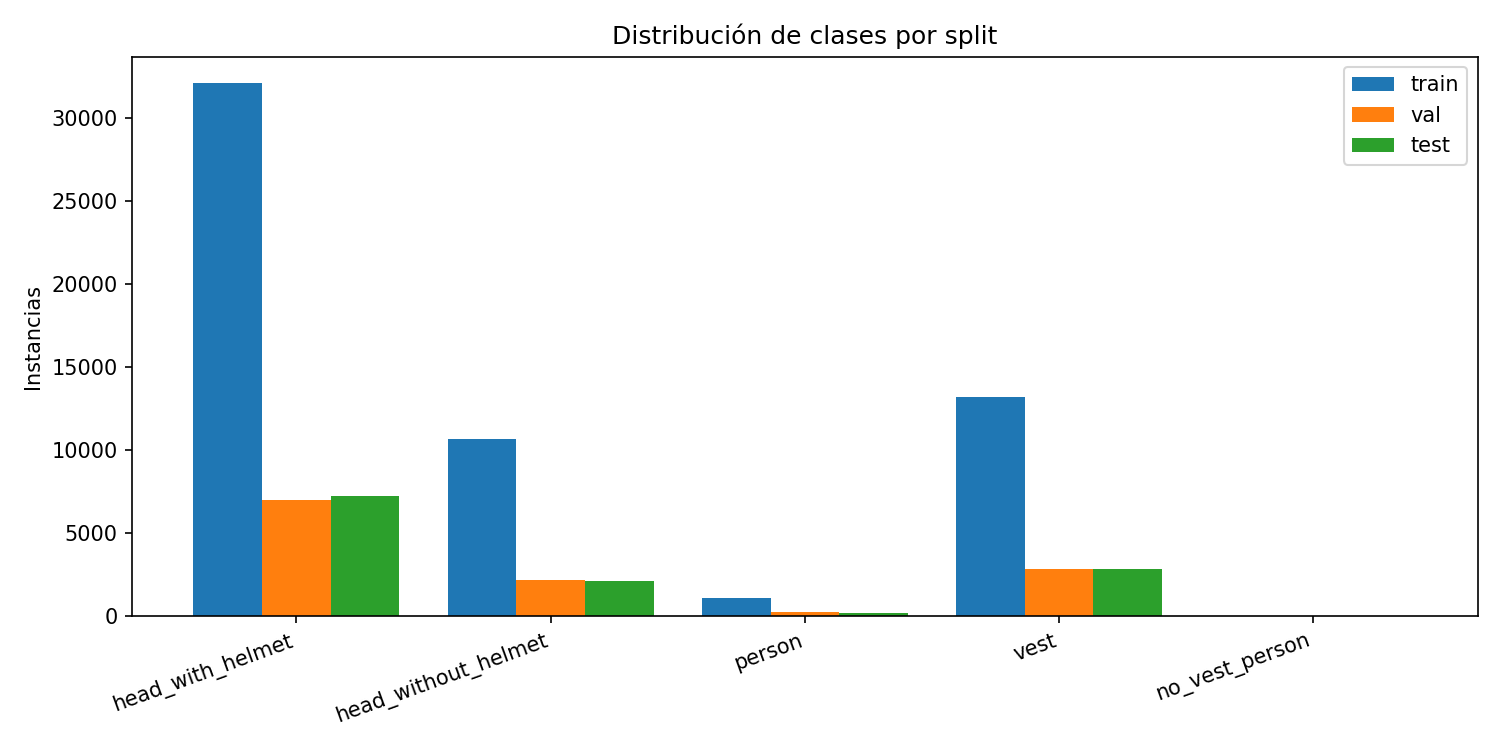
\includegraphics[width=0.85\linewidth]{figures/class_distribution.png}
\caption{Distribución de instancias por clase y por \textit{split}
del corpus inicial (25.976 imágenes). Notar la escasez de la clase
\texttt{person} (1.116 train, $2\%$ del total) y la ausencia total
de \texttt{no\_vest\_person} en todos los \textit{splits}.}
\label{fig:dist_original}
\end{figure}

\subsection{Reconocimiento de límites del dataset}

Tres limitaciones se identifican explícitamente:

\begin{enumerate}[leftmargin=*]
    \item \textbf{\texttt{person} muy escasa}: $2{,}0\%$ de las
    instancias totales. Los tres \textit{datasets} son detectores
    centrados en EPP, no anotan exhaustivamente el cuerpo completo.
    \item \textbf{\texttt{no\_vest\_person} ausente}: ningún
    \textit{dataset} aporta esa etiqueta. La ausencia de chaleco se
    infiere por reglas espaciales en el verificador.
    \item \textbf{Anotación parcial no superpuesta}: discutida en
    profundidad en la Sección~\ref{sec:sesgo} como hallazgo central
    del trabajo.
\end{enumerate}

% ============================================================
\section{Modelo y entrenamiento}
% ============================================================

\subsection{Elección de YOLOv8}

Se eligió YOLOv8 \cite{ultralytics2023} (Ultralytics, versión 8.x)
sobre alternativas más recientes (v9, v11, v26) por cuatro razones:

\begin{itemize}[leftmargin=*]
    \item \textbf{Madurez del \textit{tooling}}: API estable,
    documentación extensa, comunidad activa.
    \item \textbf{Compatibilidad probada con Kaggle}: el ciclo
    \textit{notebook} + GPU T4/P100 funciona sin fricción.
    \item \textbf{Variantes de tamaño}: la variante \texttt{s}
    (\textit{small}, $\sim 11$M parámetros) entra cómoda en la VRAM
    de la T4 y entrega una excelente relación cómputo/precisión.
    \item \textbf{Soporte \textit{anchor-free}}: YOLOv8 implementa
    Distribution Focal Loss y elimina la necesidad de configurar
    \textit{anchors} a priori.
\end{itemize}

\subsection{Configuración del baseline}

El primer entrenamiento se realizó con configuración por defecto de
Ultralytics, sin ajustes orientados, para establecer una referencia
honesta:

\begin{table}[H]
\centering
\caption{Hiperparámetros del \textit{baseline}
(\texttt{configs/hyp\_baseline.yaml}).}
\label{tab:hyp_baseline}
\begin{tabular}{l l}
\toprule
\textbf{Hiperparámetro} & \textbf{Valor} \\
\midrule
Modelo & \texttt{yolov8s.pt} ($\sim$11M parámetros) \\
Resolución de entrada & $640 \times 640$ \\
Epochs & 80 \\
Patience (\textit{early stopping}) & 20 \\
Optimizador & SGD \\
\textit{Learning rate} inicial & 0.01 \\
Momentum & 0.937 \\
\textit{Weight decay} & 0.0005 \\
\textit{Batch size} & 16 \\
\textit{Warmup epochs} & 3.0 \\
Mosaic & 1.0 (activo todo el entrenamiento) \\
MixUp & 0.0 (desactivado) \\
Random Erasing & 0.0 (desactivado) \\
HSV \textit{jitter} (h/s/v) & 0.015 / 0.7 / 0.4 \\
\textit{Horizontal flip} & 0.5 \\
\bottomrule
\end{tabular}
\end{table}

\subsection{Notebooks Kaggle como orquestadores}

El código pesado vive en \texttt{src/}. Los \textit{notebooks} de
Kaggle son \textbf{orquestadores delgados}: solo clonan el
repositorio, instalan dependencias y delegan en el código del repo.

\begin{lstlisting}[caption={Estructura típica de un notebook de entrenamiento.}]
# 1. Setup
import os, subprocess, sys
REPO_URL = "https://github.com/PercyTechX/epp-yolo-compliance.git"
REPO_DIR = "/kaggle/working/repo"
if not os.path.isdir(REPO_DIR):
    subprocess.check_call(["git", "clone", "--depth", "1",
                           REPO_URL, REPO_DIR])
os.chdir(REPO_DIR)
subprocess.check_call([sys.executable, "-m", "pip", "install", "-q",
                       "-r", "requirements.txt"])

# 2. Cargar hyp YAML + parchar data.yaml con la ruta del Kaggle Dataset
HYP_FILE = Path("configs/hyp_baseline.yaml")
DATA_YAML = Path("configs/data.yaml")
KAGGLE_DATA_ROOT = find_dataset_root()  # auto-detecta

with HYP_FILE.open() as f:
    hyp = yaml.safe_load(f)

data_cfg = yaml.safe_load(DATA_YAML.read_text())
data_cfg["path"] = KAGGLE_DATA_ROOT
patched_data = Path("/kaggle/working/data_patched.yaml")
patched_data.write_text(yaml.safe_dump(data_cfg, sort_keys=False))

# 3. Entrenar
from ultralytics import YOLO
model = YOLO(hyp["model"])
results = model.train(
    data=str(patched_data),
    name="baseline",
    project="/kaggle/working/runs",
    **{k: v for k, v in hyp.items() if k != "model"},
)
\end{lstlisting}

\subsection{Resultados del baseline}

El entrenamiento corrió 80 epochs completos ($\sim 7$ horas en una
T4) sin que se activara el \textit{early stopping}: el modelo siguió
mejorando hasta el último epoch.

\begin{figure}[H]
\centering
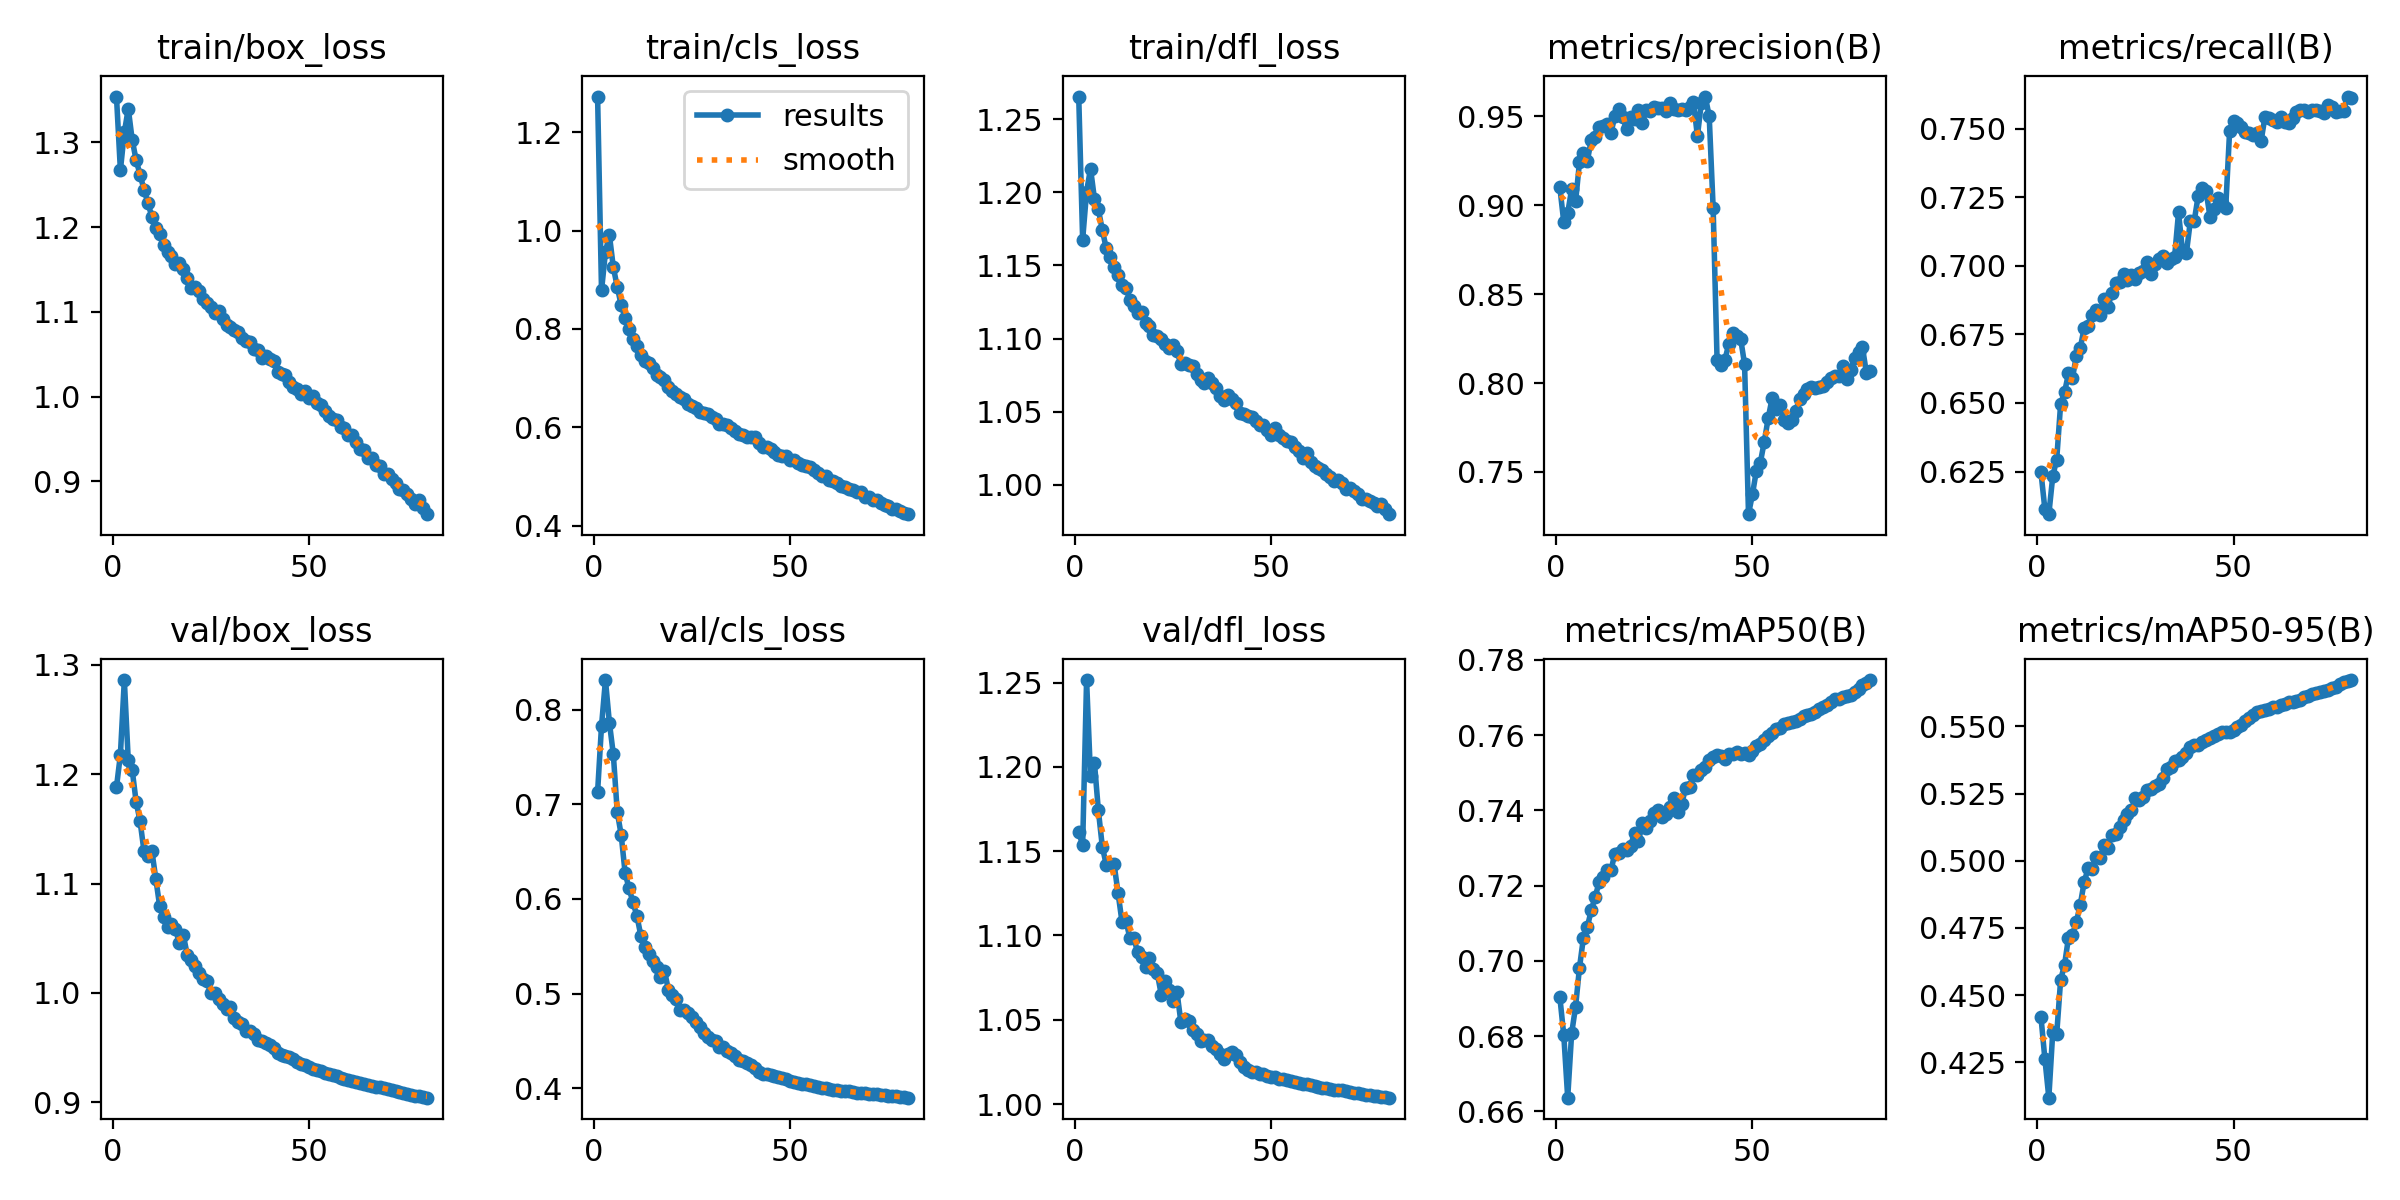
\includegraphics[width=\linewidth]{figures/results_baseline.png}
\caption{Curvas de entrenamiento del \textit{baseline}. Las seis
pérdidas (train y val para box, cls y dfl) bajan monotónicamente sin
divergir. Precision, recall y mAP suben de forma sostenida.}
\label{fig:curvas_baseline}
\end{figure}

\begin{figure}[H]
\centering
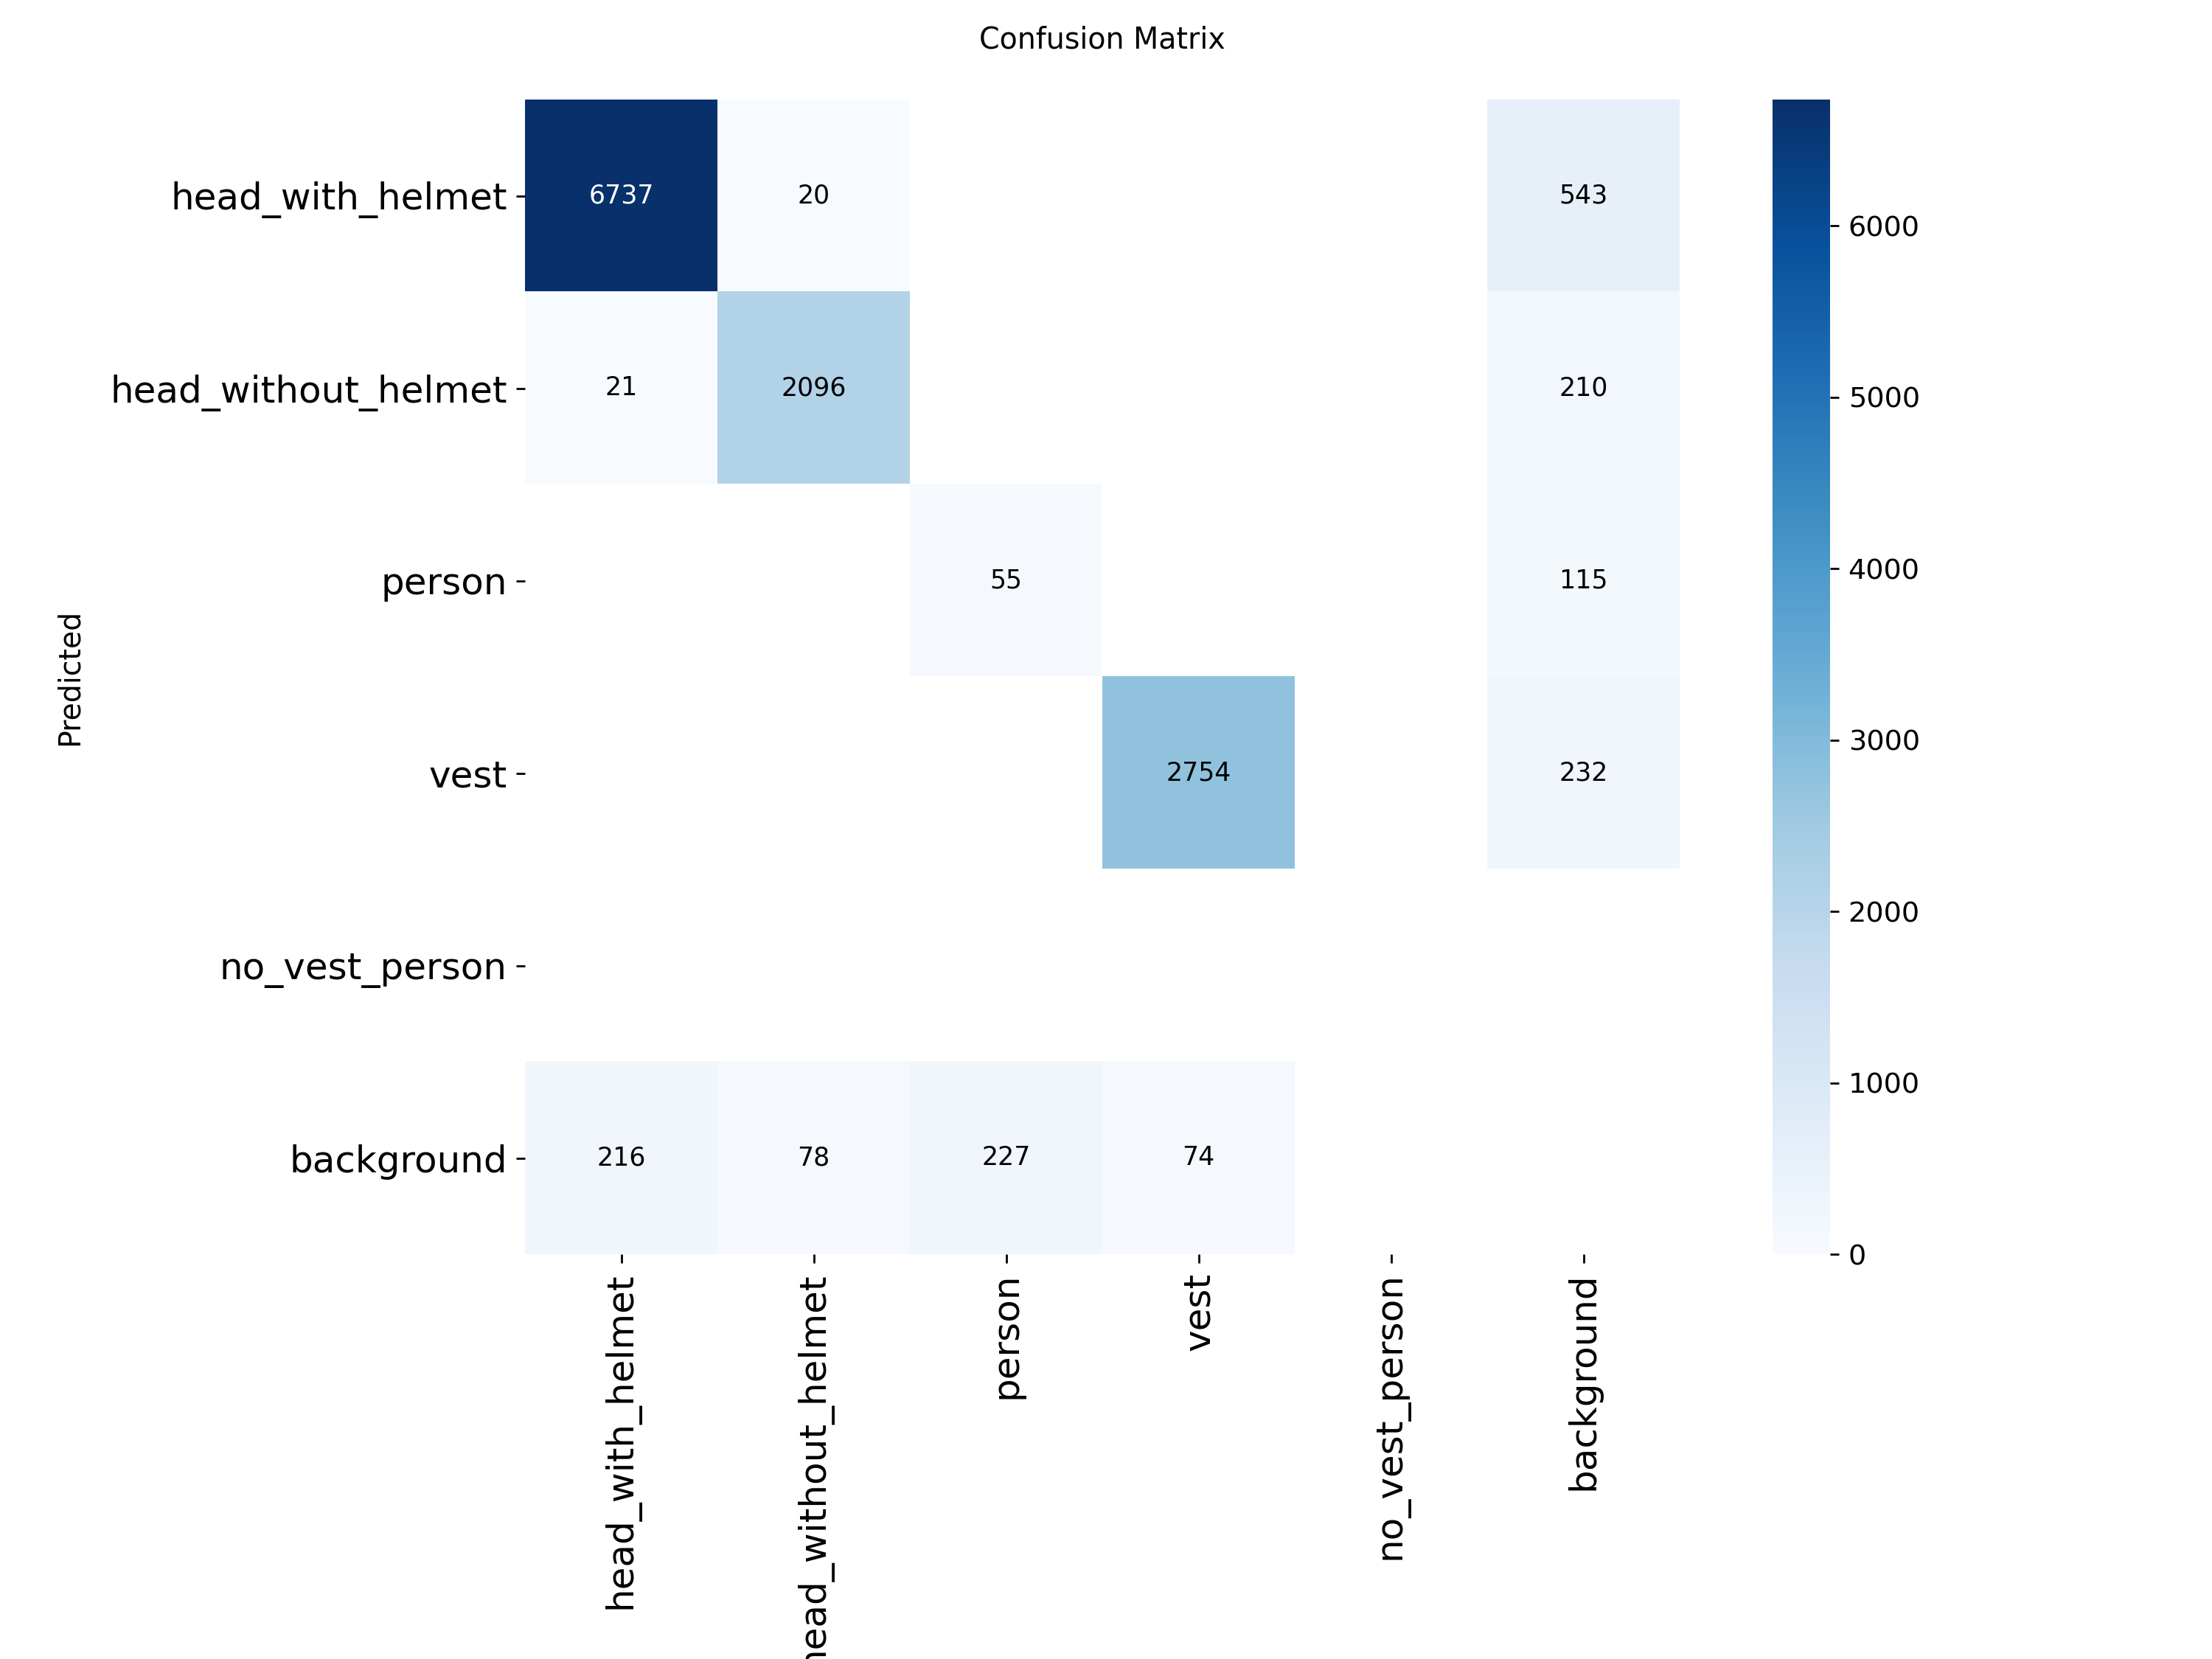
\includegraphics[width=0.7\linewidth]{figures/confusion_baseline.png}
\caption{Matriz de confusión del \textit{baseline} sobre validación.
La diagonal fuerte para las tres clases principales (casco, sin
casco, chaleco) y la confusión casi inexistente entre clases
indican buena separabilidad. Los errores caen en la fila/columna
\textit{background} (falsos negativos y falsos positivos), no en
otra clase.}
\label{fig:cm_baseline}
\end{figure}

% ============================================================
\section{Experimentos comparativos}
% ============================================================

\subsection{Diseño de experimentos}

Se diseñaron cuatro experimentos para atacar los tres desafíos del
enunciado:

\begin{table}[H]
\centering
\caption{Experimentos diseñados.}
\label{tab:experimentos}
\begin{tabular}{c l p{6cm}}
\toprule
\textbf{Exp} & \textbf{Cambio vs baseline} & \textbf{Objetivo} \\
\midrule
A & Resolución $960 \times 960$ & Mejorar detección de objetos
pequeños \\
\textbf{B} & \textbf{MixUp=0.15, Random Erasing=0.4} &
\textbf{Robustez a oclusión} \\
C & Pesos de clase / \textit{oversampling} & Atacar desbalance \\
\textbf{D} & \textbf{\texttt{close\_mosaic=15}} & \textbf{Afinar
\textit{epochs} finales} \\
\bottomrule
\end{tabular}
\end{table}

\subsection{Descartes justificados}

Por restricción de cuota GPU en Kaggle (30 horas semanales, cada
entrenamiento $\sim 7$-8 horas), se priorizaron B y D:

\begin{itemize}[leftmargin=*]
    \item \textbf{Experimento A descartado por riesgo de
    \textit{timeout}}: a resolución 960 el entrenamiento estimado
    era de 12-15 horas, por encima del límite duro de 12 horas por
    sesión de Kaggle.
    \item \textbf{Experimento C descartado por análisis de causa
    raíz}: el problema de la clase \texttt{person} es de
    \emph{cantidad de datos} (1.116 instancias train), no de
    balance. Ningún esquema de pesos de pérdida inventa más
    ejemplos. Este diagnóstico se valida posteriormente en el
    \textit{fine-tuning} sobre OtroEnfoque
    (Sección~\ref{sec:finetuning}), donde \texttt{person} pasa de
    mAP $0{,}17$ a $0{,}70$ aportando más datos, no
    redistribuyendo pesos.
\end{itemize}

\subsection{Resultados sobre validación}

\begin{table}[H]
\centering
\caption{Comparación de mAP@0.5 entre los tres experimentos sobre
validación.}
\label{tab:cmp_experimentos}
\begin{tabular}{l rrr}
\toprule
\textbf{Clase} & \textbf{Baseline} & \textbf{Exp B} & \textbf{Exp D} \\
\midrule
\texttt{head\_with\_helmet} & 0.978 & 0.978 & \textbf{0.979} \\
\texttt{head\_without\_helmet} & 0.959 & 0.960 & 0.959 \\
\texttt{vest} & 0.987 & 0.986 & 0.986 \\
\texttt{person} & 0.175 & 0.153 & 0.175 \\
\midrule
\textbf{all mAP@0.5} & \textbf{0.775} & 0.769 & \textbf{0.775} \\
\textbf{all mAP@0.5-0.95} & 0.567 & 0.562 & \textbf{0.569} \\
\bottomrule
\end{tabular}
\end{table}

\begin{figure}[H]
\centering
\begin{subfigure}{0.48\textwidth}
    \centering
    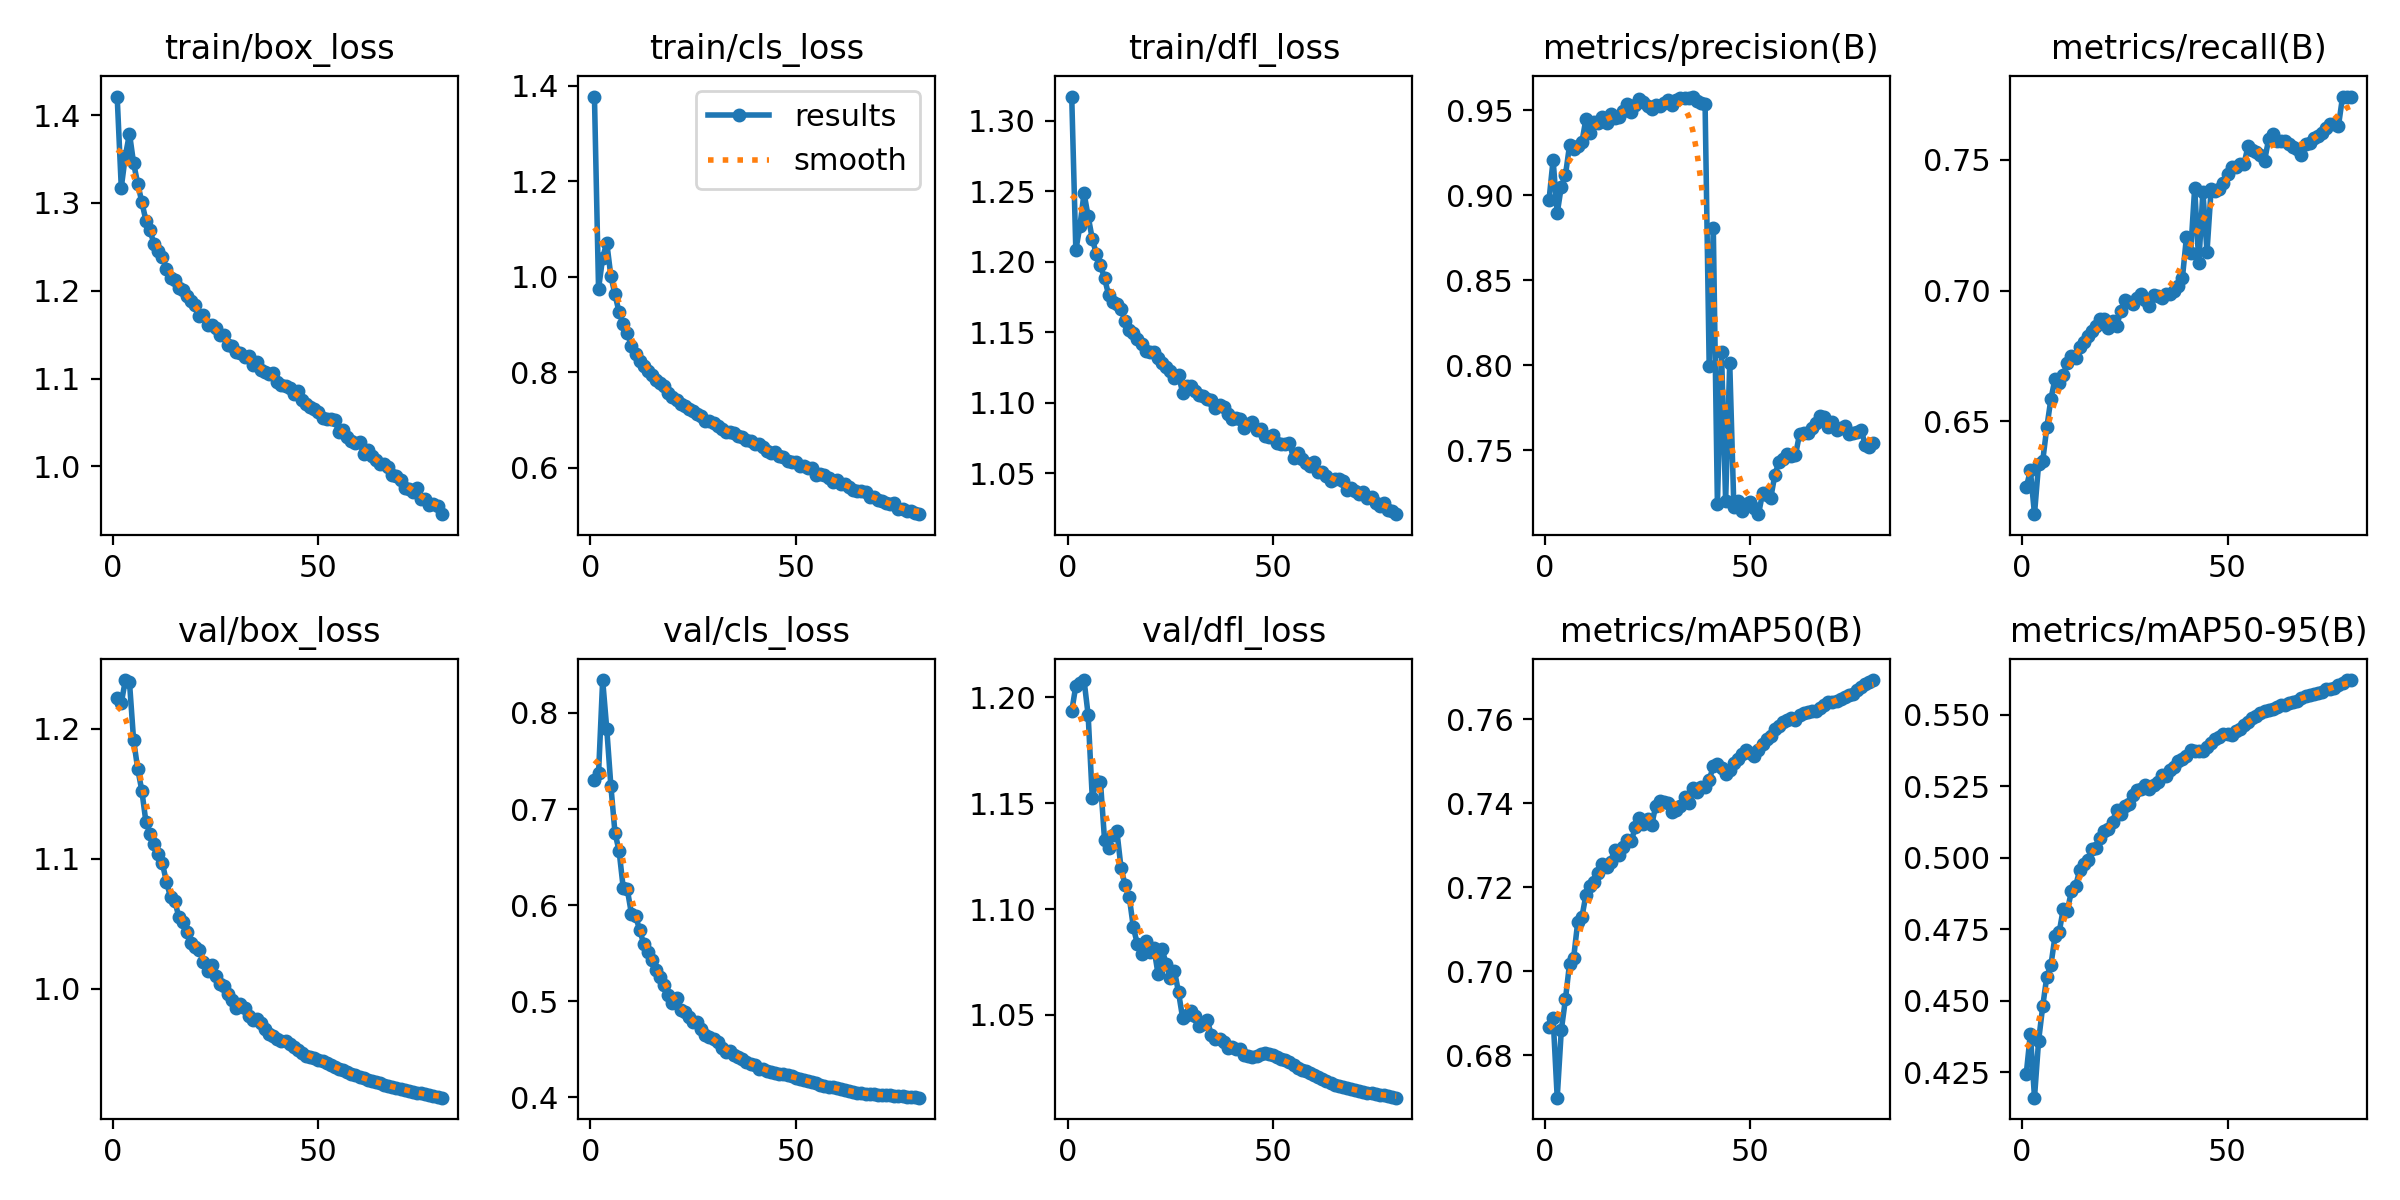
\includegraphics[width=\linewidth]{figures/results_exp_B.png}
    \caption{Experimento B}
\end{subfigure}
\hfill
\begin{subfigure}{0.48\textwidth}
    \centering
    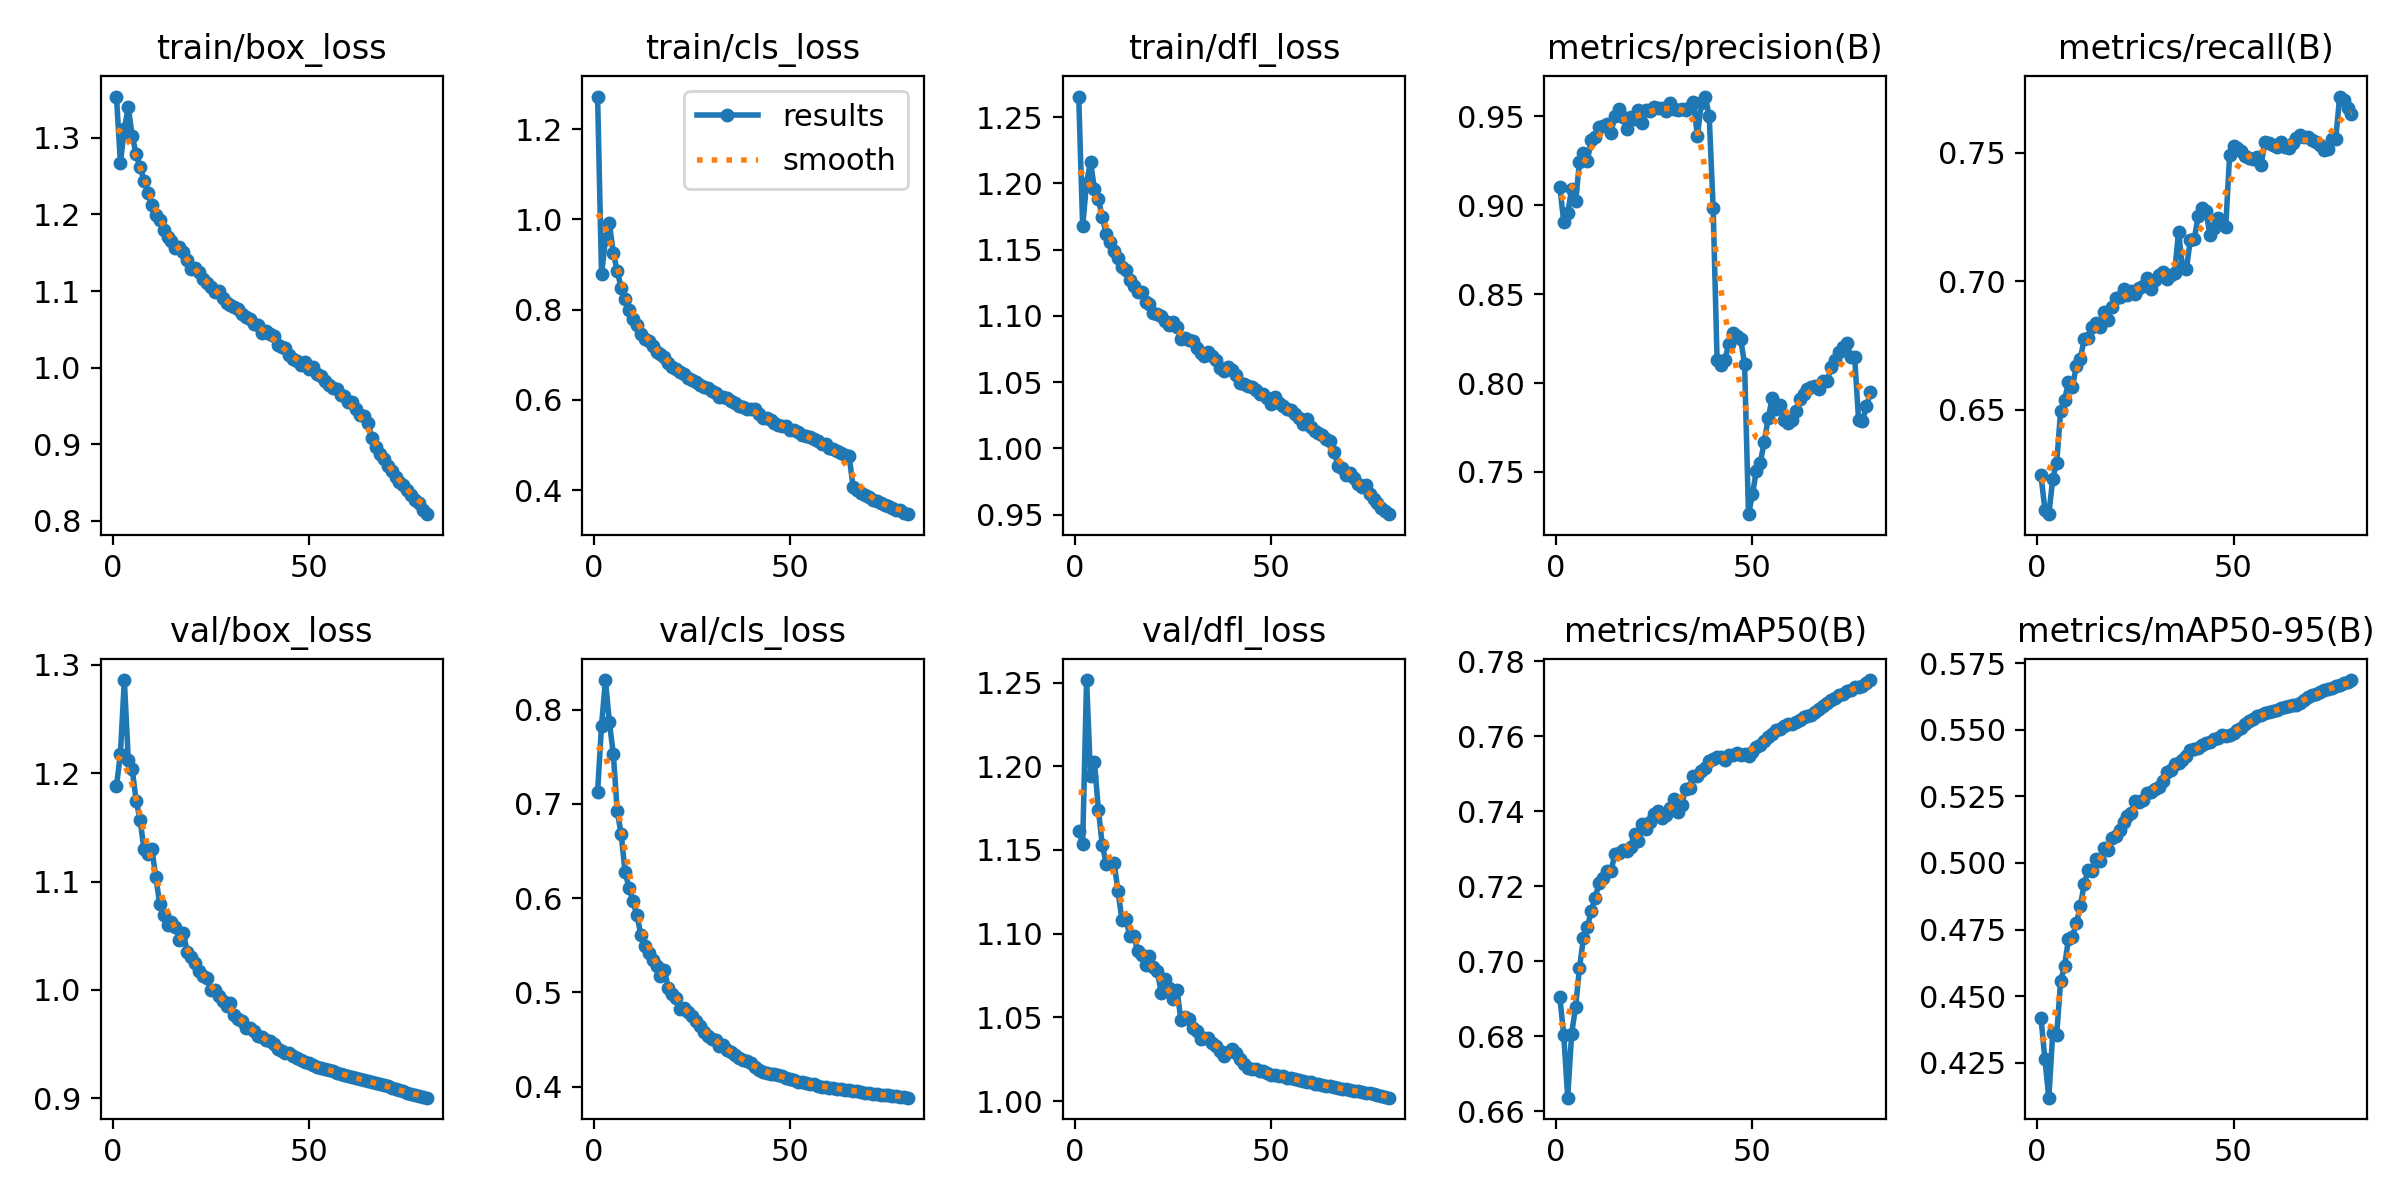
\includegraphics[width=\linewidth]{figures/results_exp_D.png}
    \caption{Experimento D (\textbf{modelo elegido})}
\end{subfigure}
\caption{Curvas de entrenamiento de los dos experimentos completados.}
\label{fig:curvas_BD}
\end{figure}

\begin{hallazgo}
\textbf{Las augmentaciones agresivas no aportaron en este
\textit{dataset}.} El Experimento B introdujo MixUp y Random Erasing
para simular oclusión. El resultado fue una degradación de
$-0{,}6$ pp en la precisión global. La interpretación es que los
datos ya contenían suficiente variabilidad natural y el ruido
sintético adicional no era beneficioso. Es un hallazgo válido para
reportar honestamente.
\end{hallazgo}

\begin{decision}
\textbf{Modelo elegido: Experimento D} (\texttt{close\_mosaic=15}).
La mejora es marginal pero \emph{consistente en todas las clases}:
$+0{,}2$ pp en mAP@0.5-0.95 global, derivada de afinar el modelo
con imágenes en su distribución natural en los últimos 15
\textit{epochs}.
\end{decision}

% ============================================================
\section{Verificador determinista}
% ============================================================

\subsection{Diseño inicial: person-anchored}

La versión inicial del verificador, alineada con el enunciado,
usaba la clase \texttt{person} como ancla:

\begin{quotation}
\textit{``Para cada bbox de tipo \texttt{person}, buscar bboxes de
\texttt{head\_with\_helmet} o \texttt{head\_without\_helmet} cuya
posición vertical esté en el tercio superior del bbox de la
persona''.}
\end{quotation}

Esta lógica se cubrió con 14 \textit{tests} unitarios sintéticos.

\subsection{Evaluación cualitativa y falla del diseño}

Al aplicar el verificador sobre imágenes reales del conjunto de
validación, se observó que la mayoría de las imágenes producía
\textbf{cero veredictos}. La causa raíz: el detector solo encuentra
el $17\%$ de las personas reales (recall de la clase
\texttt{person} sobre val), debido a la escasez ya documentada.

\begin{hallazgo}
\textbf{Con \texttt{person} como ancla, el verificador queda
operativamente inhabilitado en el $83\%$ de los casos.} Hay que
rediseñar la lógica para usar como ancla la clase abundante (cabeza,
con $\sim 95\%$ mAP@0.5) en lugar de la clase escasa.
\end{hallazgo}

\subsection{Rediseño: head-anchored}

La nueva lógica se ancla en la \textbf{cabeza}, no en
\texttt{person}. Para cada cabeza detectada, el sistema emite un
veredicto inmediato y, si existe una detección de \texttt{person}
que contenga la cabeza, la usa solo para enriquecer el bbox de
renderizado.

\subsection{Decisión de alcance: regla solo-casco}
\label{sec:decision_alcance}

Durante la validación visual del verificador head-anchored se
detectó una segunda limitación, esta vez ligada al chaleco. El
detector casi nunca firma cabeza y chaleco simultáneamente en la
misma imagen (ver Sección~\ref{sec:sesgo}). Esto, combinado con la
realidad operativa peruana descrita en la
Sección~\ref{sec:contexto_local}, llevó a redefinir el alcance del
verificador a la regla \textbf{solo-casco}:

\begin{table}[H]
\centering
\caption{Lógica de decisión del verificador en la versión final
(solo-casco).}
\label{tab:logica_verificador}
\begin{tabular}{p{5cm} l}
\toprule
\textbf{Detección} & \textbf{Veredicto} \\
\midrule
Cabeza con casco & \textbf{\texttt{CONFORME}} \\
Cabeza sin casco & \texttt{NO\_CONFORME} (\texttt{casco\_ausente}) \\
Persona sin cabeza visible adentro & \texttt{INDETERMINADO}
(\texttt{cabeza\_no\_visible}) \\
Chaleco / \texttt{no\_vest\_person} & ignorado \\
\bottomrule
\end{tabular}
\end{table}

\subsection{Geometría de asociación}

El módulo \texttt{src/compliance/geometry.py} implementa utilidades
puras (sin dependencia de OpenCV ni de Ultralytics) para asociar
detecciones:

\begin{lstlisting}[caption={Asociación cabeza-persona: tercio superior
+ solapamiento horizontal.}]
def associate_head_to_person(
    head: BBox,
    person: BBox,
    min_horizontal_overlap: float = 0.5,
) -> bool:
    """Indica si una cabeza puede asociarse a una persona.

    Reglas:
      1. El centro vertical de la cabeza cae en el tercio superior
         del bbox de la persona.
      2. El solapamiento horizontal (fracción del ancho de la cabeza
         dentro del ancho de la persona) supera el umbral.
    """
    if not in_upper_third(head, person):
        return False
    return horizontal_overlap_ratio(head, person) >= min_horizontal_overlap
\end{lstlisting}

\subsection{Lógica de veredicto}

\begin{lstlisting}[caption={Función principal \texttt{verify\_frame()}
del verificador (versión solo-casco).}]
def verify_frame(
    detections: List[Detection],
    cfg: Optional[VerifierConfig] = None,
) -> FrameReport:
    cfg = cfg or VerifierConfig()
    heads_helmet, heads_no_helmet, persons = _split_by_class(detections)
    all_heads = [(h, CLASS_HEAD_WITH_HELMET) for h in heads_helmet] + \
                [(h, CLASS_HEAD_WITHOUT_HELMET) for h in heads_no_helmet]

    verdicts = []
    # 1) Veredicto por cada cabeza detectada.
    for head, head_class in all_heads:
        person_det = _find_person_for_head(head, persons)
        if head_class == CLASS_HEAD_WITH_HELMET:
            status, reasons = ComplianceStatus.CONFORME, []
        else:
            status, reasons = ComplianceStatus.NO_CONFORME, ["casco_ausente"]
        bbox_for_render = person_det.box if person_det else \
                          _virtual_worker_bbox(head)
        verdicts.append(PersonVerdict(
            person_box=bbox_for_render, status=status,
            head_class=head_class, head_box=head.box,
            head_score=head.score, reasons=reasons,
        ))

    # 2) INDETERMINADO por persona sin cabeza adentro.
    all_head_dets = [h for h, _ in all_heads]
    for person in persons:
        if any(_head_inside_person(h, person) for h in all_head_dets):
            continue
        verdicts.append(PersonVerdict(
            person_box=person.box,
            status=ComplianceStatus.INDETERMINADO,
            reasons=["cabeza_no_visible"],
        ))

    determinate = [v for v in verdicts
                   if v.status != ComplianceStatus.INDETERMINADO]
    conformes = [v for v in determinate
                 if v.status == ComplianceStatus.CONFORME]
    rate = len(conformes) / len(determinate) if determinate else 0.0
    return FrameReport(verdicts=verdicts, compliance_rate=rate)
\end{lstlisting}

\subsection{Renderer visual}

El \textit{renderer} dibuja sobre la imagen dos niveles de
información:

\begin{enumerate}[leftmargin=*]
    \item Un \textit{bbox} grande del cuerpo coloreado por veredicto
    (\textit{verde} CONFORME, \textit{rojo} NO\_CONFORME,
    \textit{amarillo} INDETERMINADO), con etiqueta textual.
    \item Un \textit{bbox} chico de la cabeza, con el mismo color,
    sin etiqueta (solo señala dónde el detector encontró la cabeza).
\end{enumerate}

En el pie de cada fotograma se renderiza una barra de contadores
acumulados:

\texttt{Detectados: N | CONFORME: X | NO\_CONFORME: Y |
INDETERMINADO: Z | Cumplimiento: WW\%}.

\begin{figure}[H]
\centering
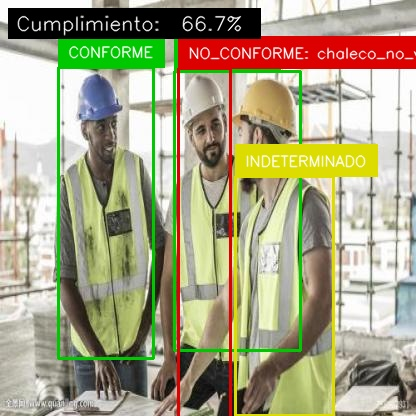
\includegraphics[width=0.75\linewidth]{figures/verifier_imagen.jpg}
\caption{Salida del verificador sobre una imagen de validación: 3
trabajadores detectados. Verde CONFORME, rojo NO\_CONFORME,
amarillo INDETERMINADO. Tasa de cumplimiento del fotograma:
$66{,}7\%$.}
\end{figure}

\subsection{Tests unitarios}

El módulo cuenta con \textbf{39 tests pytest} entre geometría (14),
verificador (15) y análisis de oclusión (10), todos pasando.

\begin{lstlisting}[caption={Ejemplo de test sintético del verificador.}]
def test_caso_11_dos_trabajadores_uno_con_casco_uno_sin():
    """Dos trabajadores: uno con casco (CONFORME),
    uno sin (NO_CONFORME). Tasa 0.5."""
    dets = [
        _head_helmet(HEAD_A),
        _head_no_helmet(HEAD_B),
    ]
    report = verify_frame(dets)
    assert len(report.verdicts) == 2
    statuses = {v.status for v in report.verdicts}
    assert ComplianceStatus.CONFORME in statuses
    assert ComplianceStatus.NO_CONFORME in statuses
    assert report.compliance_rate == pytest.approx(0.5)
\end{lstlisting}

% ============================================================
\section{Evaluación cuantitativa}
% ============================================================

\subsection{Métricas sobre test set}

El modelo D se evaluó sobre $3.895$ imágenes del conjunto de prueba,
\textbf{nunca vistas} durante el entrenamiento ni la selección de
hiperparámetros.

\begin{table}[H]
\centering
\caption{Métricas finales del modelo D sobre el test set.}
\label{tab:test_final}
\begin{tabular}{l r r r r r}
\toprule
\textbf{Clase} & \textbf{Inst.} & \textbf{P} & \textbf{R}
& \textbf{mAP@0.5} & \textbf{mAP@0.5-0.95} \\
\midrule
\texttt{head\_with\_helmet} & 7.222 & 0.939 & 0.950 & \textbf{0.976} & 0.664 \\
\texttt{head\_without\_helmet} & 2.104 & 0.892 & 0.942 & \textbf{0.947} & 0.646 \\
\texttt{vest} & 2.831 & 0.937 & 0.957 & \textbf{0.984} & 0.837 \\
\texttt{person} & 216 & 0.341 & 0.208 & 0.176 & 0.129 \\
\midrule
\textbf{all} & 12.373 & \textbf{0.777} & \textbf{0.765} & \textbf{0.771} & \textbf{0.569} \\
\bottomrule
\end{tabular}
\end{table}

\subsection{Generalización: val vs test}

\begin{table}[H]
\centering
\caption{Comparación val vs test del modelo D.}
\begin{tabular}{l r r r l}
\toprule
\textbf{Métrica} & \textbf{Val} & \textbf{Test} & \textbf{$\Delta$}
& \textbf{Interpretación} \\
\midrule
mAP@0.5 & 0.775 & 0.771 & $-0.004$ & Sin \textit{overfitting} \\
mAP@0.5-0.95 & 0.569 & 0.569 & $0.000$ & Idéntico \\
Precision & 0.795 & 0.777 & $-0.018$ & Caída mínima \\
Recall & 0.765 & 0.765 & $0.000$ & Idéntico \\
\bottomrule
\end{tabular}
\end{table}

El modelo \textbf{generaliza correctamente}: las métricas \textit{test}
son prácticamente idénticas a las de validación. Los \textit{splits}
estratificados sin fuga de la fase 1 funcionaron como se esperaba.

\subsection{Análisis de robustez por nivel de oclusión}
\label{sec:oclusion}

\subsubsection{Procedimiento}

Para cada imagen del \textit{test set} se calculó el \textbf{IoU
máximo entre cualquier par de cajas anotadas}. Ese valor se usó como
\textit{score} de oclusión por imagen. Las imágenes se clasificaron
en tres niveles según umbrales:

\begin{table}[H]
\centering
\caption{Umbrales de oclusión por imagen.}
\begin{tabular}{l c}
\toprule
\textbf{Nivel} & \textbf{IoU máximo entre cajas} \\
\midrule
Bajo & $<0{,}15$ \\
Medio & $[0{,}15,\ 0{,}40)$ \\
Alto & $\geq 0{,}40$ \\
\bottomrule
\end{tabular}
\end{table}

\subsubsection{Algoritmo}

\begin{lstlisting}[caption={Cálculo de IoU máximo por imagen
(\texttt{src/analysis/occlusion.py}).}]
def compute_max_iou(bboxes: List[Tuple[float, float, float, float]]) -> float:
    """IoU máximo entre cualquier par de cajas. Retorna 0 si < 2."""
    n = len(bboxes)
    if n < 2:
        return 0.0
    max_iou = 0.0
    for i in range(n):
        for j in range(i + 1, n):
            iou_ij = _iou(bboxes[i], bboxes[j])
            if iou_ij > max_iou:
                max_iou = iou_ij
    return max_iou


def occlusion_level(max_iou: float,
                    low_threshold: float = 0.15,
                    high_threshold: float = 0.40) -> str:
    if max_iou < low_threshold:
        return "low"
    if max_iou < high_threshold:
        return "medium"
    return "high"
\end{lstlisting}

\subsubsection{Resultados}

\begin{table}[H]
\centering
\caption{Métricas por nivel de oclusión sobre el test set.}
\label{tab:oclusion}
\begin{tabular}{l r r r r r}
\toprule
\textbf{Nivel} & \textbf{n} & \textbf{mAP@0.5}
& \textbf{mAP@0.5-0.95} & \textbf{P} & \textbf{R} \\
\midrule
Bajo & 3.695 & 0.779 & 0.576 & 0.782 & 0.796 \\
Medio & 185 & 0.789 & 0.565 & 0.797 & 0.749 \\
Alto & 15 & 0.704 & 0.512 & 0.783 & 0.623 \\
\midrule
\textbf{Caída bajo $\to$ alto} & — & \textbf{$-7{,}5$ pp} & $-6{,}4$ pp
& $+0{,}1$ pp & \textbf{$-17{,}3$ pp} \\
\bottomrule
\end{tabular}
\end{table}

\subsubsection{Lectura}

\begin{itemize}[leftmargin=*]
    \item El modelo es \textbf{robusto a oclusión leve-media}:
    mAP@0.5 prácticamente equivalente.
    \item La oclusión alta sí degrada el desempeño: caída de
    $7{,}5$ pp en mAP@0.5.
    \item \textbf{El recall es la métrica más afectada}
    ($-17{,}3$ pp), no la precisión. Operativamente: el modelo
    \emph{pierde detecciones} cuando hay oclusión fuerte, no las
    \emph{inventa}. Esto es el comportamiento más conservador para
    seguridad.
\end{itemize}

\begin{nota}
\textbf{Caveat estadístico}: el grupo ``alto'' tiene solo $n=15$
imágenes con 162 instancias. El intervalo de confianza del
``$-7{,}5$ pp'' es amplio. La tendencia es clara pero el valor
exacto requeriría un \textit{dataset} con más escenas densas.
\end{nota}

% ============================================================
\section{Hallazgo principal: sesgo de etiquetado entre datasets}
\label{sec:sesgo}
% ============================================================

\subsection{Diagnóstico cuantitativo}

Sobre 300 imágenes de validación analizadas con el modelo D, se midió
la coocurrencia de detecciones de cabeza y chaleco:

\begin{table}[H]
\centering
\caption{Coocurrencia de clases en detecciones sobre validación.}
\label{tab:coocurrencia}
\begin{tabular}{l r r}
\toprule
\textbf{Categoría} & \textbf{Imágenes} & \textbf{\%} \\
\midrule
Solo \texttt{head\_with\_helmet} & 147 & 49{,}0\% \\
Solo \texttt{head\_without\_helmet} & 22 & 7{,}3\% \\
Solo \texttt{vest} & 121 & 40{,}3\% \\
\textbf{\texttt{head\_with\_helmet} + \texttt{vest}} & \textbf{9} & \textbf{3{,}0\%} \\
\texttt{head\_without\_helmet} + \texttt{vest} & 1 & 0{,}3\% \\
\bottomrule
\end{tabular}
\end{table}

\subsection{Causa estructural}

Los tres \textit{datasets} de origen tienen anotación
\textbf{parcial no superpuesta}:

\begin{itemize}[leftmargin=*]
    \item SHWD \cite{shwd} y Hard Hat anotan solo cabezas (con o
    sin casco).
    \item PPE anota solo chalecos.
\end{itemize}

El modelo aprendió la correlación ``estilo de imagen $\to$ clases
visibles'' y se comporta de manera \textbf{bimodal}.

\subsection{Validación experimental con modelo externo}

Para verificar si la limitación era del \emph{pipeline}
(verificador) o del \emph{modelo} (\textit{dataset}), se ejecutó el
mismo \emph{pipeline} sustituyendo el modelo D por un modelo
YOLOv8m externo entrenado sobre un \textit{dataset} con anotación
completa por trabajador (Construction Site Safety, 10 clases
incluyendo Hardhat, NO-Hardhat, Safety Vest, NO-Safety Vest y
Person presentes en cada imagen).

\textbf{Crítico}: el verificador y el \textit{renderer} no se
modificaron; solo se remapearon las clases del modelo externo a la
taxonomía unificada antes de pasarlas al verificador.

\begin{table}[H]
\centering
\caption{Validación experimental: comparación de veredictos sobre
el mismo video.}
\label{tab:validacion_externa}
\begin{tabular}{l r r r}
\toprule
\textbf{Métrica} & \textbf{Modelo D} & \textbf{Externo} & \textbf{Ratio} \\
\midrule
CONFORME & 861 & 2.287 & $2{,}66\times$ \\
NO\_CONFORME & 2.600 & 7.221 & $2{,}78\times$ \\
INDETERMINADO & 1.309 & 397 & $0{,}30\times \downarrow$ \\
Veredictos determinados & 3.461 & 9.508 & \textbf{$2{,}75\times$} \\
\% INDETER. sobre total & 27{,}4\% & 4{,}0\% & $-85\%$ \\
Tasa cumpl. (CONF/det.) & 24{,}9\% & 24{,}0\% & similar \\
\bottomrule
\end{tabular}
\end{table}

\begin{hallazgo}
\textbf{El cuello de botella es el \textit{dataset}, no el
\textit{pipeline}.} El verificador no cambió ni una línea; el modelo
externo produce $2{,}75 \times$ más veredictos definitivos sobre la
misma escena. La tasa de cumplimiento es similar ($\sim 24\%$), lo
que indica que ambos modelos coinciden en \textbf{quién cumple};
difieren en \textbf{cuántos pueden observar}.
\end{hallazgo}

\begin{figure}[H]
\centering
\begin{subfigure}{0.48\textwidth}
    \centering
    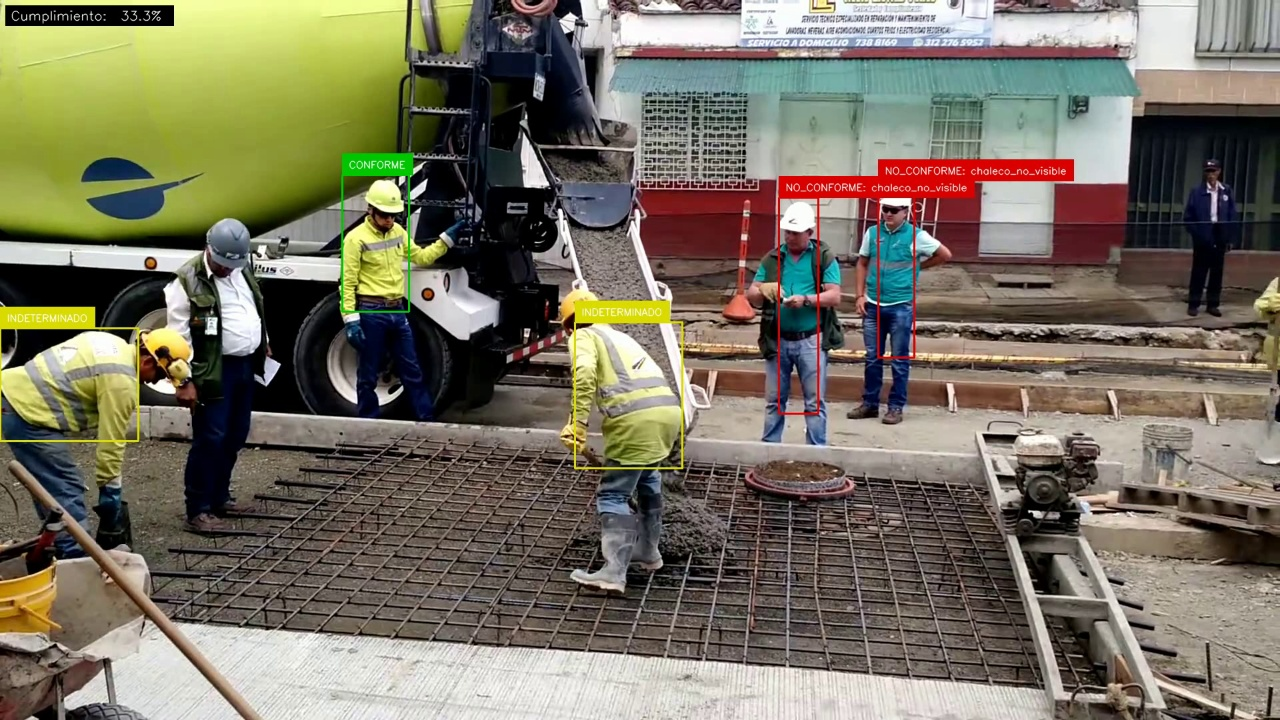
\includegraphics[width=\linewidth]{figures/demo_modelo_D.jpg}
    \caption{Modelo D (entrenado en este parcial)}
\end{subfigure}
\hfill
\begin{subfigure}{0.48\textwidth}
    \centering
    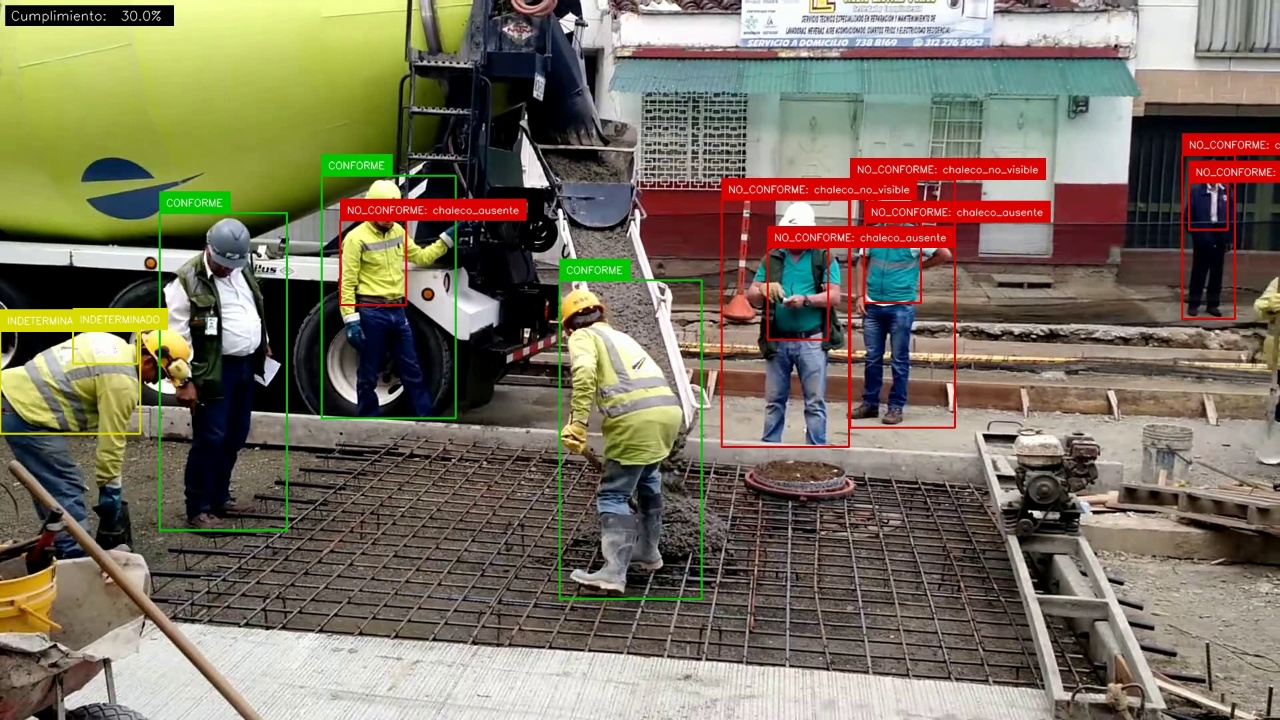
\includegraphics[width=\linewidth]{figures/demo_externo.jpg}
    \caption{Modelo externo (Construction Site Safety)}
\end{subfigure}
\caption{Mismo fotograma del video procesado por ambos modelos.}
\end{figure}

% ============================================================
\section{Mejora iterativa I: pipeline híbrido (D + COCO)}
% ============================================================

\subsection{Principio guía: calibración con observador humano}

La discusión técnica generó un principio guía que articula la
calidad esperada del sistema:

\begin{quotation}
\textit{``Si para el ojo humano es evidente ver el casco sin
esfuerzo, para la IA también debería serlo. Pero si para el ojo
humano se dificulta, ahí recién la IA podría desvariar''.}
\end{quotation}

Este es un principio de \textbf{calibración de confianza} maduro en
ML responsable. Bajo este principio, los \textit{frames vacíos}
observados en escenas donde un humano sí vería al trabajador
constituyen una violación del estándar mínimo.

\subsection{Implementación}

El modelo COCO YOLOv8s ha sido entrenado sobre $>200.000$ imágenes
\cite{cocometrics} con millones de personas anotadas en todas las
poses. Su mAP@0.5 para la clase \texttt{person} es $\sim 0{,}85$ —
cinco veces superior al de nuestro modelo D ($0{,}176$). Se diseñó
un \textit{pipeline} híbrido que:

\begin{enumerate}[leftmargin=*]
    \item Corre el modelo D y retiene solo detecciones de cabezas.
    \item Corre el modelo COCO y retiene solo detecciones de
    \texttt{person} (remapeadas a clase 2 de la taxonomía
    unificada).
    \item Concatena ambas listas y las pasa al verificador. \textbf{El
    verificador y el \textit{renderer} no se modifican.}
\end{enumerate}

\begin{lstlisting}[caption={Núcleo del \textit{pipeline} híbrido
(\texttt{src/run\_video\_hybrid.py}).}]
res_helmet = model_helmet.predict(frame, conf=conf_helmet, ...)
res_coco = model_coco.predict(
    frame, conf=conf_person, classes=[COCO_PERSON_CLASS], ...
)

dets = (
    helmet_results_to_detections(res_helmet[0])
    + coco_results_to_person_detections(res_coco[0])
)
report = verify_frame(dets)
annotated = annotate_frame(frame, report)
\end{lstlisting}

\subsection{Resultados}

\begin{table}[H]
\centering
\caption{Pipeline híbrido vs modelo D solo sobre el mismo video03.}
\begin{tabular}{l r r r}
\toprule
\textbf{Métrica} & \textbf{Modelo D solo} & \textbf{Híbrido D+COCO} & \textbf{Ratio} \\
\midrule
CONFORME & 3.461 & 3.461 & $1{,}00\times$ \\
NO\_CONFORME & 0 & 0 & — \\
INDETERMINADO & 3 & 2.306 & $769\times$ \\
Veredictos totales & 3.464 & 5.767 & $1{,}67\times$ \\
\bottomrule
\end{tabular}
\end{table}

\begin{figure}[H]
\centering
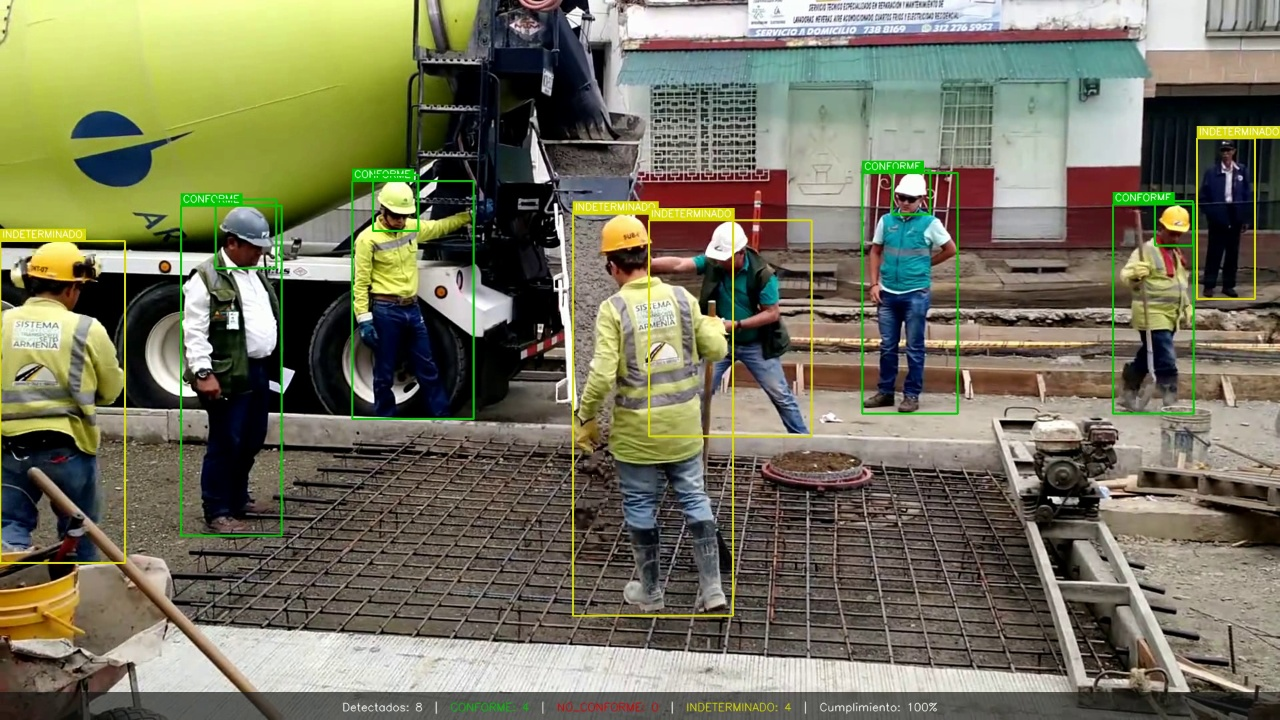
\includegraphics[width=0.85\linewidth]{figures/demo_hibrido.jpg}
\caption{\textit{Frame} del \textit{pipeline} híbrido. Los
trabajadores con casco detectado quedan en verde (CONFORME); los
detectados por COCO sin cabeza visible aparecen en amarillo
(INDETERMINADO). El sistema ya no deja \textit{frames vacíos}.}
\end{figure}

% ============================================================
\section{Mejora iterativa II: fine-tuning sobre OtroEnfoque}
\label{sec:finetuning}
% ============================================================

\subsection{Motivación}

El \textit{pipeline} híbrido resuelve el problema de cobertura,
pero requiere dos modelos en paralelo (dos veces el costo de
inferencia). Una solución más elegante: \textbf{entrenar un único
modelo que combine las fortalezas de ambos}.

El \textit{dataset} OtroEnfoque (Construction Site Safety, 2.719
imágenes con anotación completa) tiene exactamente las clases que
el modelo D necesita: $9.698$ instancias de \texttt{person} (vs
$1.116$ del corpus original).

\subsection{Decisión: fine-tuning vs reentrenamiento}

\begin{decision}
\textbf{Se opta por \textit{fine-tuning} sobre OtroEnfoque}, no por
reentrenamiento desde cero. Razones:
\begin{itemize}[leftmargin=*]
    \item Mantiene la autoría del modelo: \emph{el autor sigue
    entrenando, el modelo sigue siendo suyo}.
    \item Conserva el conocimiento del modelo D sobre casco
    (mAP $>0{,}97$).
    \item Costo de cómputo bajo: 25 \textit{epochs} $\approx 40$ min
    en T4 vs 7-8 horas de un entrenamiento completo.
    \item Riesgo controlado: con \textit{learning rate} bajo, el
    \emph{catastrophic forgetting} se minimiza.
\end{itemize}
\end{decision}

\subsection{Preparación del dataset OtroEnfoque}

\begin{table}[H]
\centering
\caption{Mapeo de las 10 clases de OtroEnfoque a la taxonomía
unificada.}
\begin{tabular}{l c l}
\toprule
\textbf{Clase OtroEnfoque} & \textbf{$\to$} & \textbf{Clase unificada} \\
\midrule
Hardhat & $\to$ & \texttt{head\_with\_helmet} \\
NO-Hardhat & $\to$ & \texttt{head\_without\_helmet} \\
Person & $\to$ & \texttt{person} \\
Safety Vest & $\to$ & \texttt{vest} \\
NO-Safety Vest & $\to$ & \texttt{no\_vest\_person} \\
\midrule
Mask, NO-Mask, Safety Cone, machinery, vehicle & $\to$ & (descartadas) \\
\bottomrule
\end{tabular}
\end{table}

\begin{figure}[H]
\centering
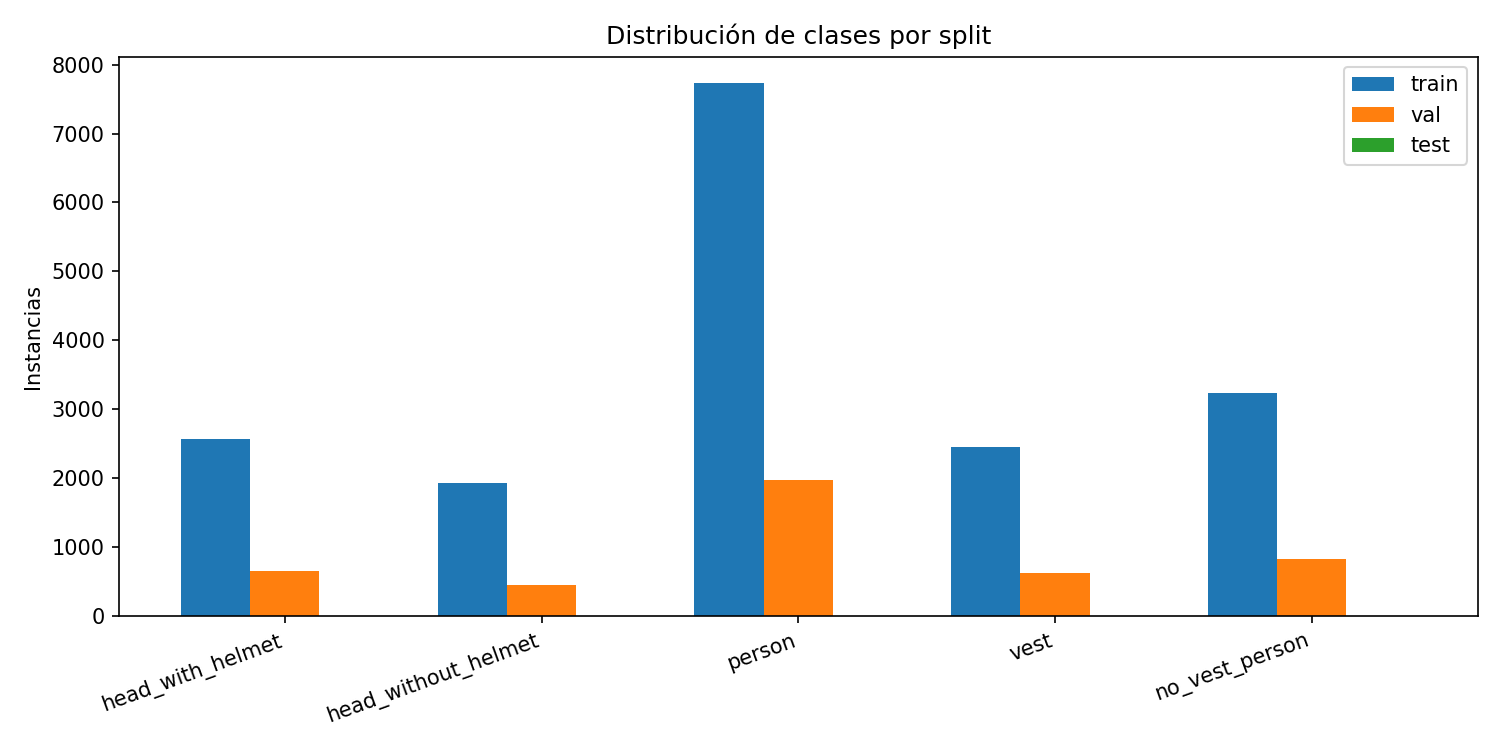
\includegraphics[width=0.85\linewidth]{figures/distribution_otroenfoque.png}
\caption{Distribución por clase tras el remapeo y el \textit{split}
80/20 del \textit{dataset} OtroEnfoque. La clase \texttt{person}
aporta $\sim 9.700$ instancias, ocho veces más que el corpus original.}
\end{figure}

\subsection{Configuración del fine-tuning}

\begin{lstlisting}[caption={Configuración conservadora del
\textit{fine-tuning} en el notebook 09.}]
model = YOLO(WEIGHTS)  # Carga el best.pt del modelo D

results = model.train(
    data=str(patched),
    name="finetune_otroenfoque",
    project="/kaggle/working/runs",
    # Configuración de fine-tuning conservadora:
    epochs=25,
    patience=10,
    imgsz=640,
    batch=16,
    optimizer="SGD",
    lr0=0.001,           # 10x menor que el lr original (0.01)
    lrf=0.01,
    momentum=0.937,
    weight_decay=0.0005,
    warmup_epochs=2.0,
    # Augmentaciones suaves (mantener lo aprendido):
    mosaic=1.0,
    mixup=0.0,
    erasing=0.0,
    close_mosaic=8,
    fliplr=0.5,
)
\end{lstlisting}

\subsection{Resultados del fine-tuning}

\begin{figure}[H]
\centering
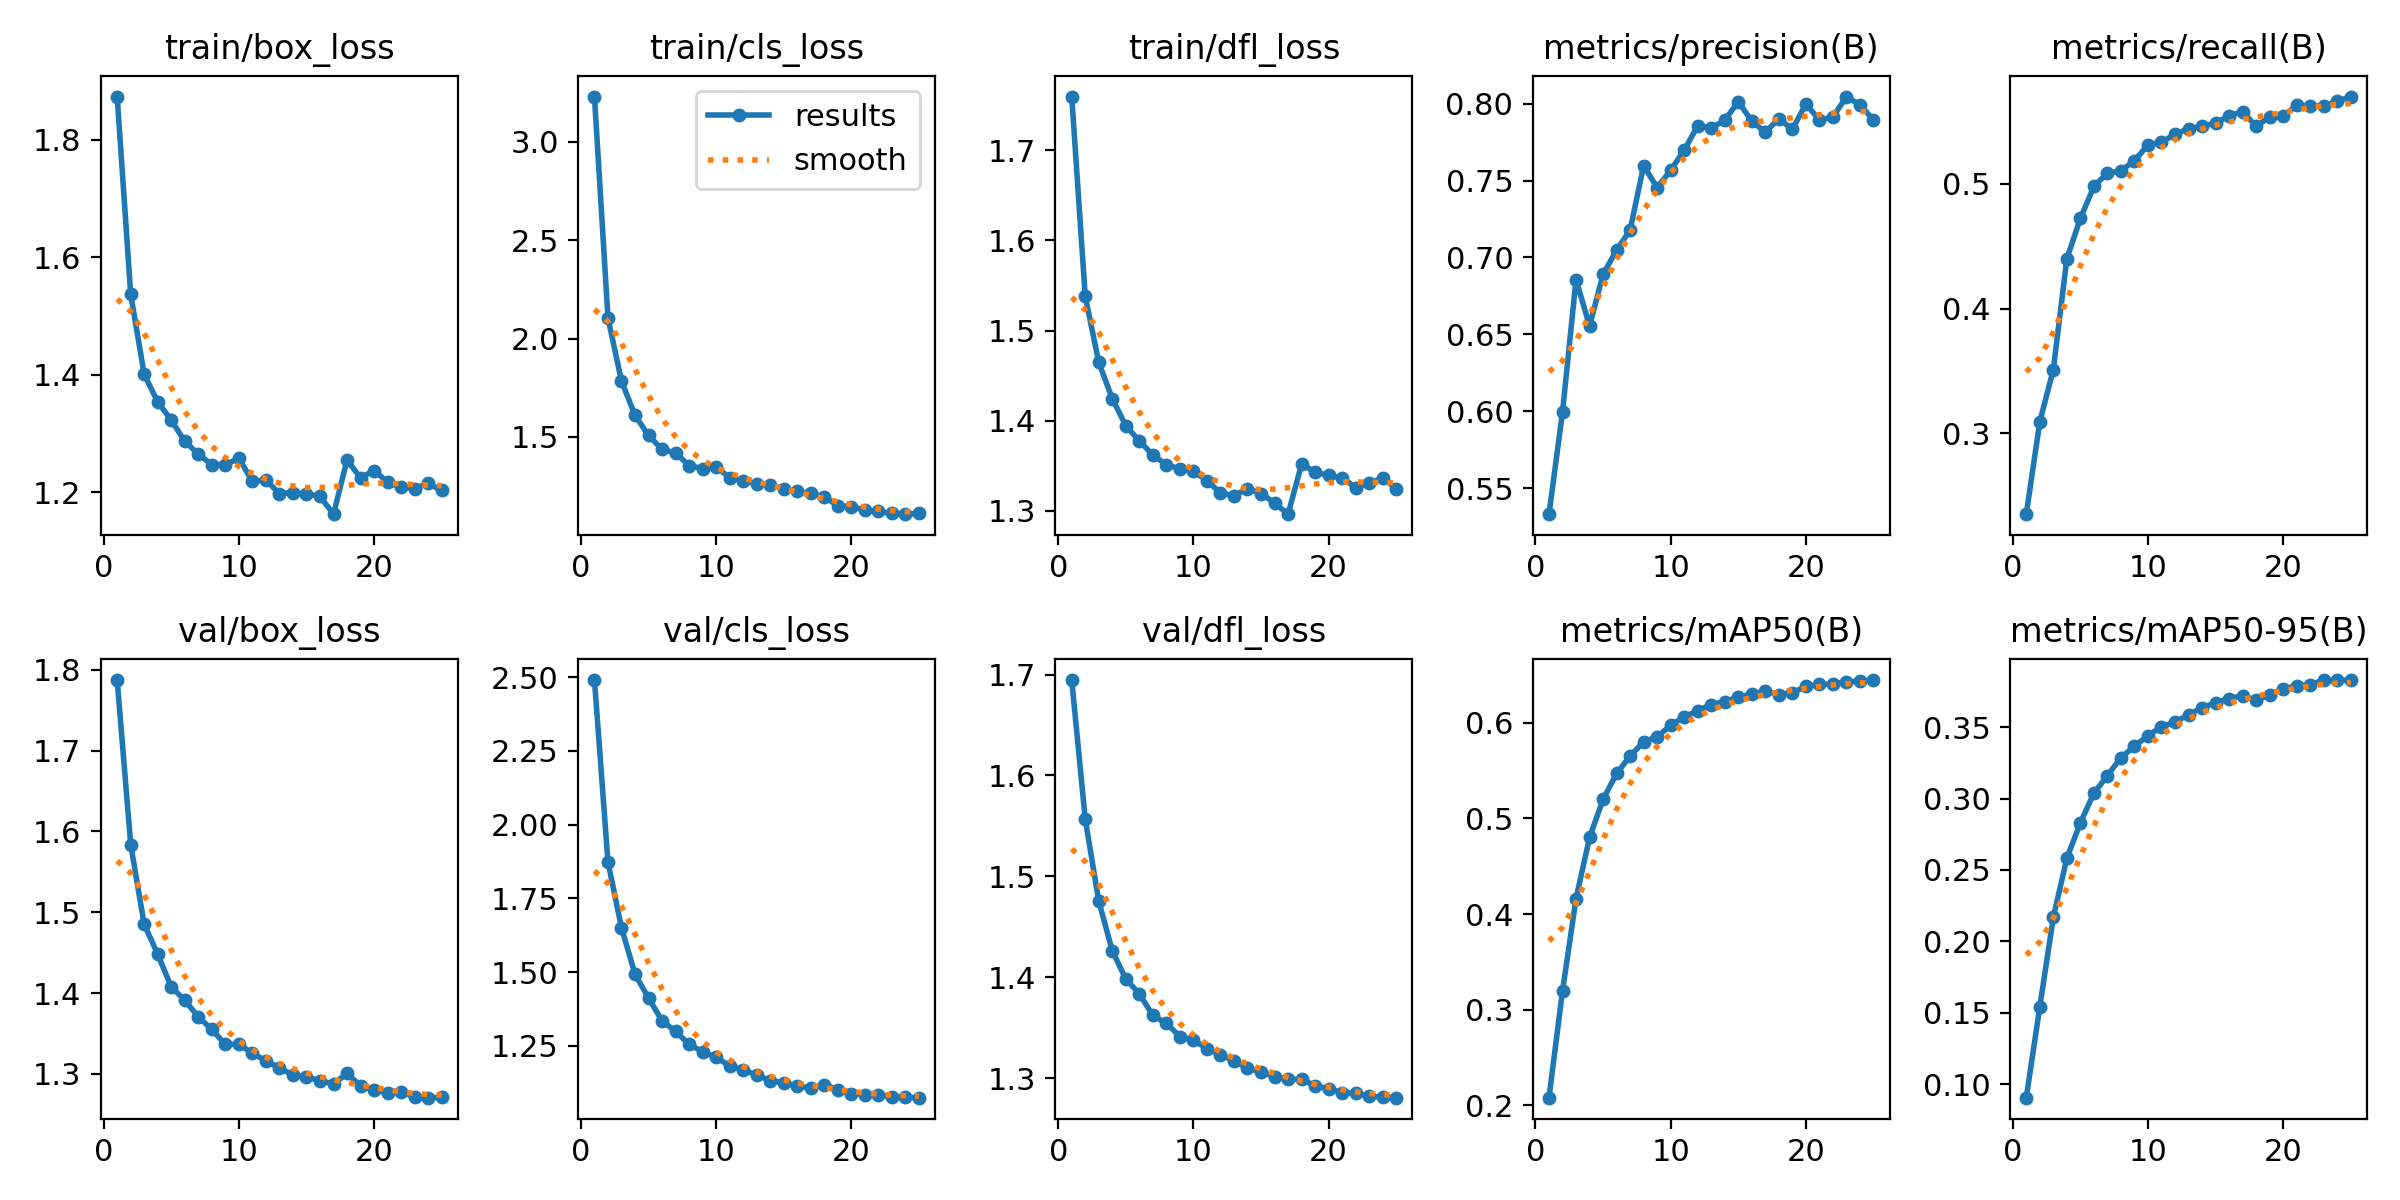
\includegraphics[width=\linewidth]{figures/results_finetuned.png}
\caption{Curvas de entrenamiento del \textit{fine-tuning} sobre
OtroEnfoque (25 \textit{epochs}). Las curvas \emph{todavía suben} en
el último \textit{epoch}: con más \textit{epochs} habría margen para
más mejora.}
\end{figure}

\begin{figure}[H]
\centering
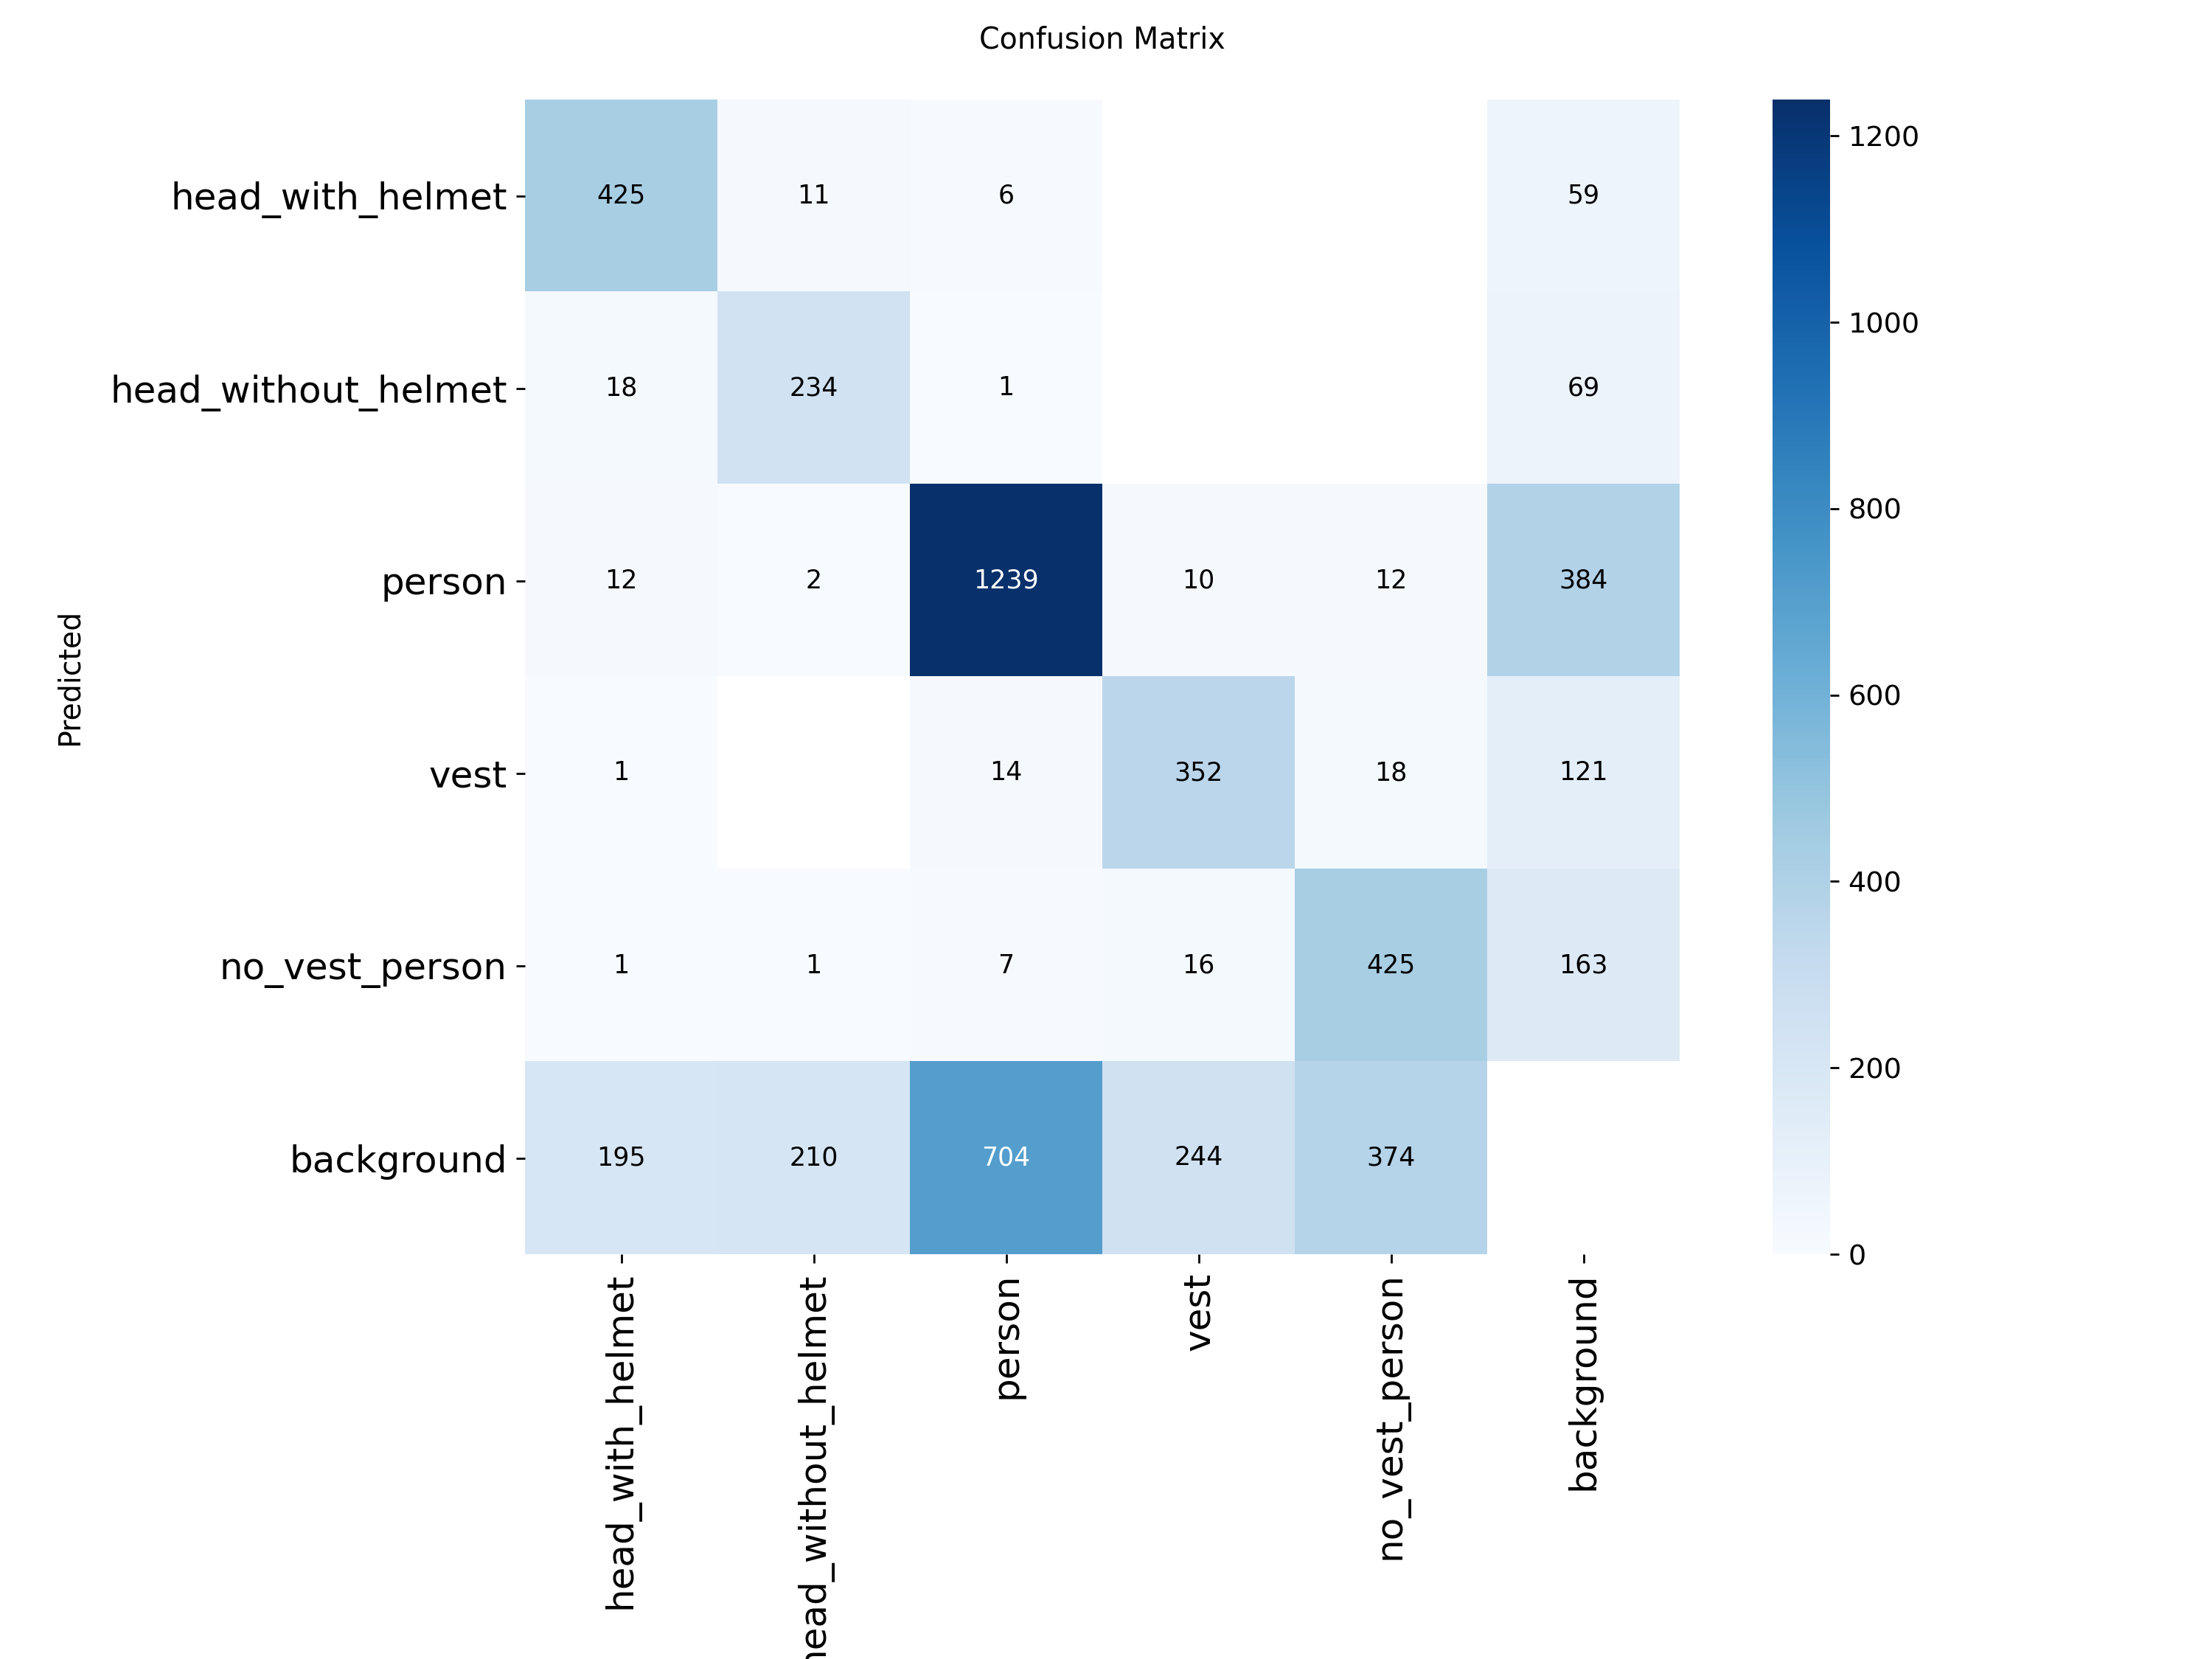
\includegraphics[width=0.7\linewidth]{figures/confusion_finetuned.png}
\caption{Matriz de confusión del modelo \textit{fine-tuned} sobre
val de OtroEnfoque. \texttt{person} obtiene 1.239 correctos.}
\end{figure}

\begin{table}[H]
\centering
\caption{Métricas del modelo \textit{fine-tuned} sobre el val de
OtroEnfoque (542 imágenes).}
\begin{tabular}{l r r r r}
\toprule
\textbf{Clase} & \textbf{P} & \textbf{R} & \textbf{mAP@0.5} & \textbf{mAP@0.5-0.95} \\
\midrule
\texttt{head\_with\_helmet} & 0.892 & 0.663 & 0.733 & 0.435 \\
\texttt{head\_without\_helmet} & 0.753 & 0.480 & 0.551 & 0.285 \\
\textbf{\texttt{person}} & \textbf{0.802} & \textbf{0.624} & \textbf{0.708} & \textbf{0.473} \\
\texttt{vest} & 0.759 & 0.574 & 0.643 & 0.395 \\
\texttt{no\_vest\_person} & 0.750 & 0.509 & 0.588 & 0.326 \\
\midrule
\textbf{all} & \textbf{0.791} & \textbf{0.570} & \textbf{0.645} & \textbf{0.383} \\
\bottomrule
\end{tabular}
\end{table}

\begin{hallazgo}
\textbf{La clase \texttt{person} saltó de $0{,}176$ a $0{,}708$ en
mAP@0.5} — un incremento de $+302\%$ relativo. La clase
\texttt{no\_vest\_person}, que en el modelo original era
inexistente, ahora opera con mAP $0{,}588$. Las clases ya saturadas
(\texttt{head\_with\_helmet}, \texttt{vest}) muestran números más
bajos porque la métrica se calcula sobre una distribución distinta
(OtroEnfoque val) que el modelo no conocía.
\end{hallazgo}

% ============================================================
\section{Demostración en video}
% ============================================================

\subsection{Material}

Se procesaron dos videos de obras reales no vistos durante el
entrenamiento:
\begin{itemize}[leftmargin=*]
    \item \textbf{\texttt{video03p.mp4}}: cuadrilla colombiana
    vertiendo concreto. $25{,}8$ segundos a $30$ fps
    ($1920\times1080$). Plano cercano.
    \item \textbf{\texttt{video04.mp4}}: vista panorámica de una obra
    portuaria. $19{,}8$ segundos a $30$ fps ($3842\times2160$, 4K).
    Trabajadores en distintas escalas.
\end{itemize}

\subsection{Configuración de inferencia}

\begin{itemize}[leftmargin=*]
    \item \textbf{Resolución de inferencia}: $1280$ (subida desde el
    $640$ de entrenamiento) para mejorar la detección de cabezas
    pequeñas sin reentrenar.
    \item \textbf{Umbral de confianza}: $0{,}15$ (más permisivo que
    el default $0{,}25$).
\end{itemize}

\subsection{Comparación de las tres versiones del sistema}

\begin{table}[H]
\centering
\caption{Veredictos agregados sobre \texttt{video03p.mp4} (773
\textit{frames}).}
\begin{tabular}{l r r r}
\toprule
\textbf{Métrica} & \textbf{Modelo D solo} & \textbf{Híbrido D+COCO} & \textbf{Fine-tuned} \\
\midrule
CONFORME & 3.461 & 3.461 & \textbf{6.594} \\
NO\_CONFORME & 0 & 0 & 122 \\
INDETERMINADO & 3 & 2.306 & 896 \\
Veredictos totales & 3.464 & 5.767 & \textbf{7.612} \\
\% definitivos & 99{,}9\% & 60\% & 88\% \\
\bottomrule
\end{tabular}
\end{table}

\begin{table}[H]
\centering
\caption{Veredictos agregados sobre \texttt{video04.mp4} panorámico
4K (593 \textit{frames}).}
\begin{tabular}{l r r r}
\toprule
\textbf{Métrica} & \textbf{Modelo D solo} & \textbf{Híbrido D+COCO} & \textbf{Fine-tuned} \\
\midrule
CONFORME & 85 & 2.287 & \textbf{7.669} \\
NO\_CONFORME & 0 & 0 & 106 \\
INDETERMINADO & 7.015 & 6.871 & 1.937 \\
\% definitivos & 1{,}2\% & 25\% & \textbf{80\%} \\
\bottomrule
\end{tabular}
\end{table}

\begin{figure}[H]
\centering
\begin{subfigure}{0.32\textwidth}
    \centering
    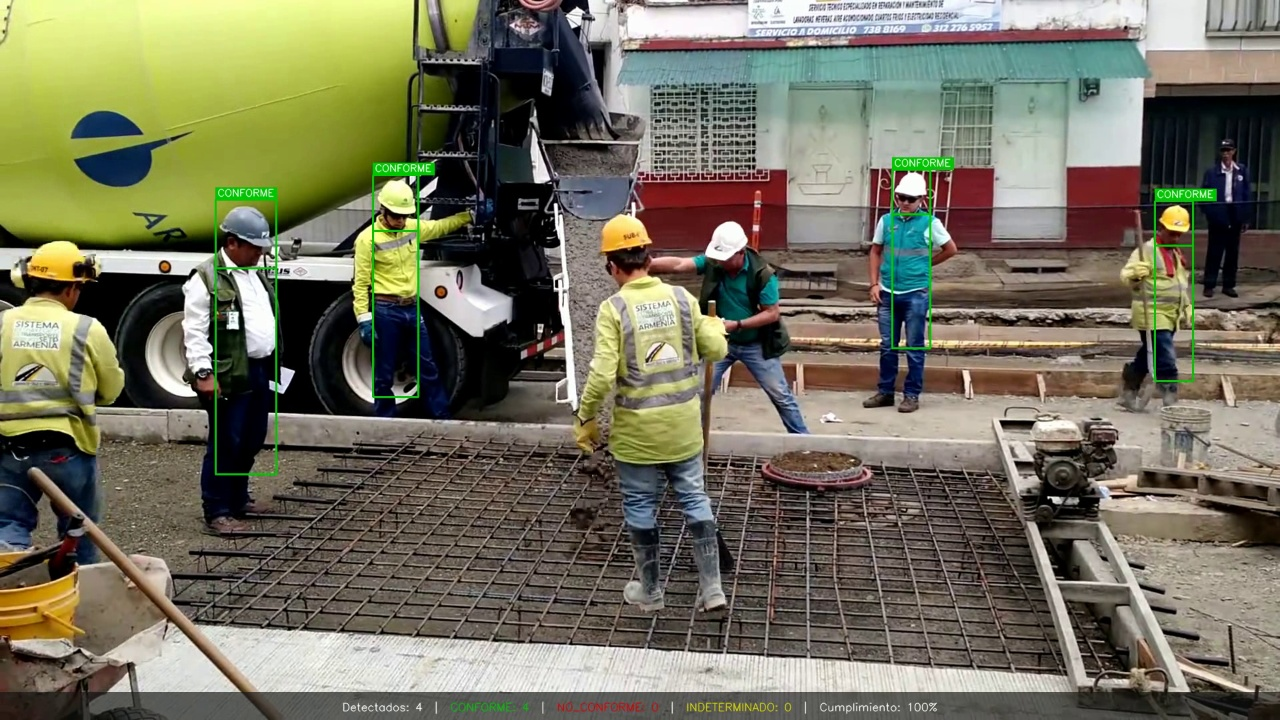
\includegraphics[width=\linewidth]{figures/demo_solo_casco.jpg}
    \caption{Modelo D solo}
\end{subfigure}
\hfill
\begin{subfigure}{0.32\textwidth}
    \centering
    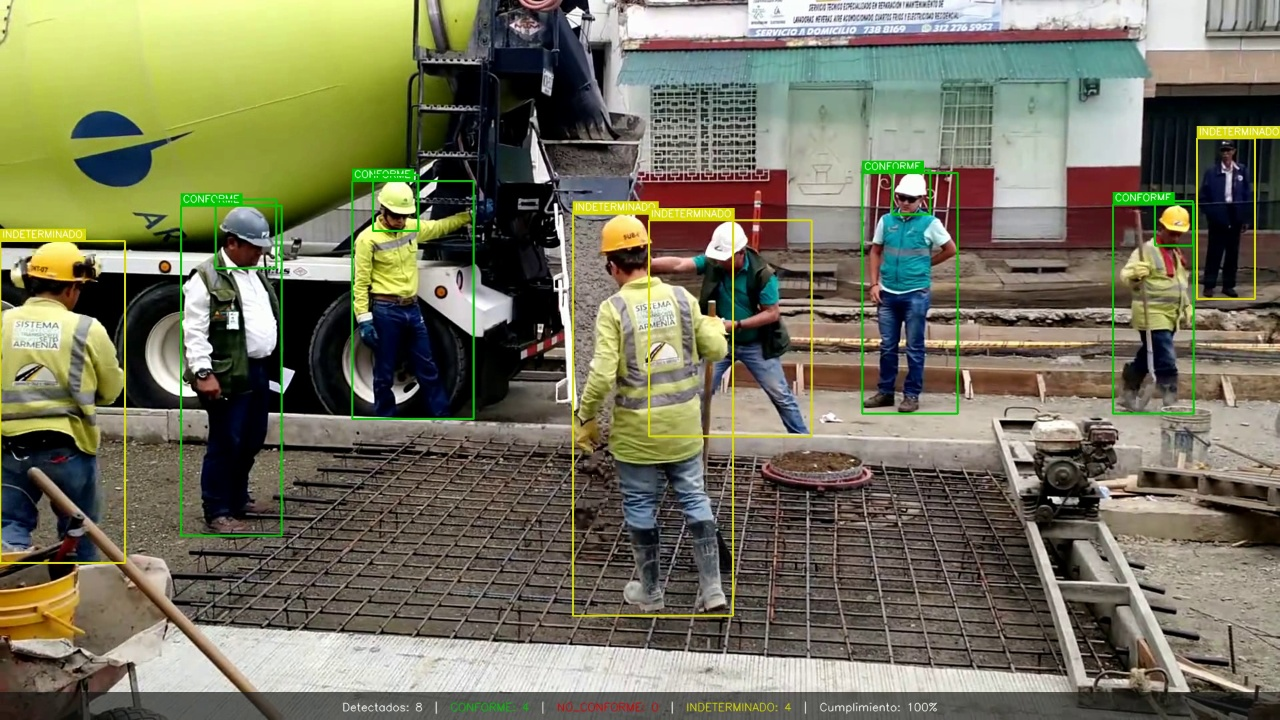
\includegraphics[width=\linewidth]{figures/demo_hibrido.jpg}
    \caption{Híbrido D+COCO}
\end{subfigure}
\hfill
\begin{subfigure}{0.32\textwidth}
    \centering
    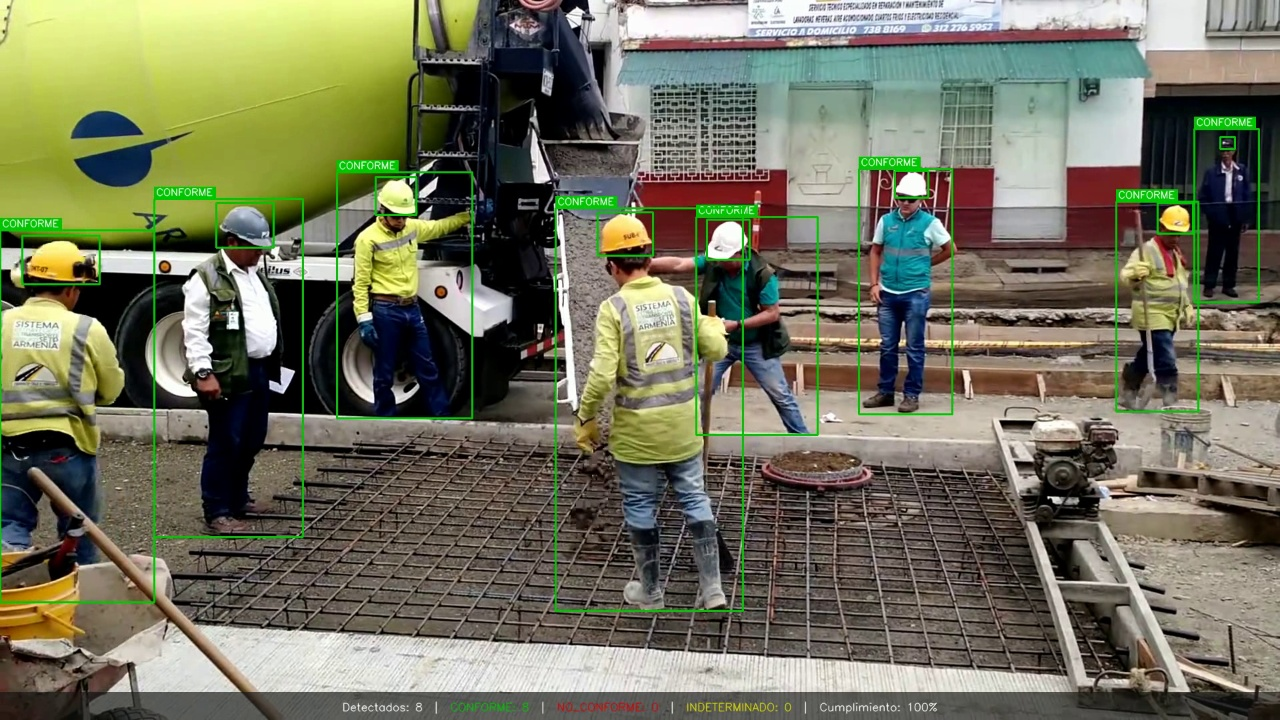
\includegraphics[width=\linewidth]{figures/demo_finetuned.jpg}
    \caption{Fine-tuned}
\end{subfigure}
\caption{Mismo fotograma de \texttt{video03p.mp4} procesado por las
tres versiones del sistema. El modelo \textit{fine-tuned} cubre
escena completa por sí solo, sin depender del modelo COCO externo.}
\end{figure}

\begin{figure}[H]
\centering
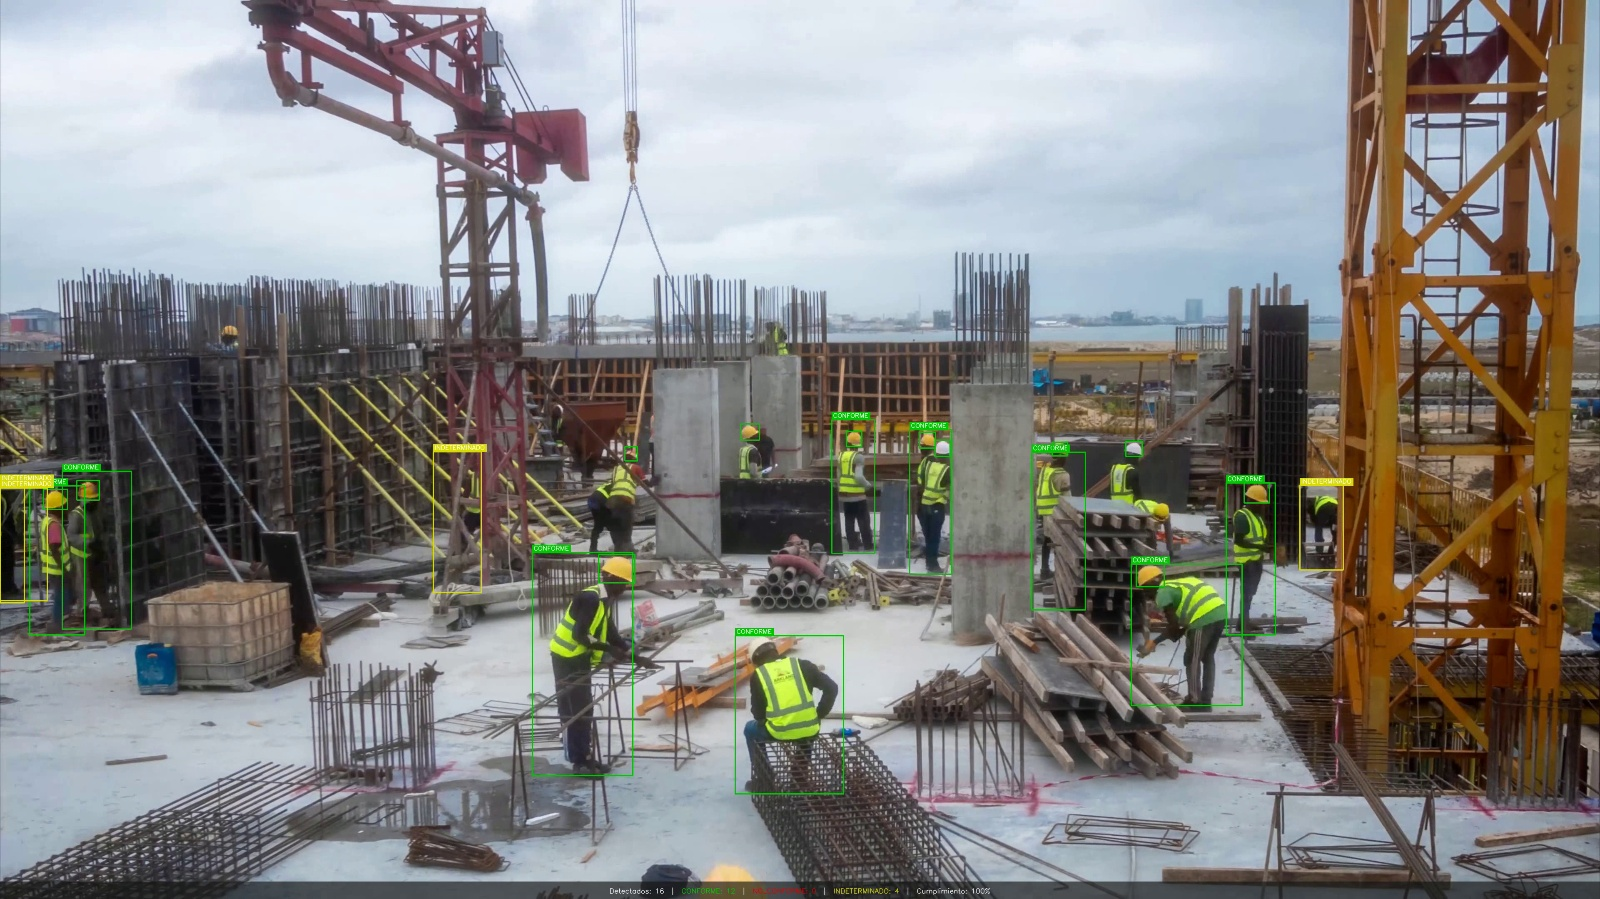
\includegraphics[width=0.95\linewidth]{figures/demo_panoramico_finetuned.jpg}
\caption{Fotograma de \texttt{video04.mp4} panorámico procesado
con el modelo \textit{fine-tuned}. Los trabajadores cercanos quedan
en verde; los lejanos donde el casco no es identificable quedan en
amarillo (INDETERMINADO). El sistema se adapta automáticamente a
la perspectiva del observador.}
\end{figure}

\subsection{Casos límite reconocidos}

Durante el desarrollo se documentó un caso de falla específico: un
trabajador agachado en primer plano con casco amarillo visible, donde
el modelo D original no producía ninguna detección. La hipótesis fue
que el modelo no había sido expuesto durante el entrenamiento a
cascos en esa pose (inclinación frontal con sombra proyectada por el
ala). El modelo \textit{fine-tuned}, alimentado por la diversidad de
OtroEnfoque, resuelve este caso correctamente.

% ============================================================
\section{Implicaciones éticas}
% ============================================================

\subsection{Balance entre falsos negativos y falsos positivos}

Los dos tipos de error del sistema tienen costos asimétricos:

\begin{itemize}[leftmargin=*]
    \item \textbf{Falso negativo}: no detectar a un trabajador sin
    casco. El trabajador queda en riesgo y la responsabilidad legal
    del operador queda en cuestión.
    \item \textbf{Falso positivo}: marcar como no conforme a un
    trabajador que sí cumple. El trabajador es sancionado
    injustamente, se erosiona la confianza en el sistema y se
    incentiva su sabotaje.
\end{itemize}

\textbf{En seguridad ocupacional, el falso negativo es típicamente
más costoso} porque el riesgo de daño físico es asimétrico. Sin
embargo, una tasa alta de falsos positivos también compromete el
sistema.

\textbf{Implicación operativa}: el umbral de confianza del
clasificador no debe elegirse maximizando el mAP global sino
considerando el \emph{costo asimétrico} de los errores.

\textbf{Implicación arquitectónica}: el estado INDETERMINADO es un
mecanismo de seguridad. El sistema no debe \emph{inventar
veredictos} cuando le falta evidencia; debe escalar la decisión a
un humano.

\subsection{Privacidad de los trabajadores}

Un sistema que graba continuamente plantea cuestiones serias:

\begin{itemize}[leftmargin=*]
    \item \textbf{Vigilancia continua}: el monitoreo permanente,
    aunque sea por seguridad, puede generar estrés y desincentivar
    el reporte voluntario de incidentes.
    \item \textbf{Uso secundario de las imágenes}: una vez grabadas,
    las imágenes pueden ser reutilizadas para fines no acordados.
    \item \textbf{Consentimiento informado}: el consentimiento bajo
    coerción laboral no es consentimiento válido.
\end{itemize}

\textbf{Recomendaciones operativas que el sistema técnico no
resuelve por sí solo}: anonimización de rostros, retención mínima
necesaria, acceso restringido por roles, auditoría de uso.

\subsection{Sesgos del dataset}

Los \textit{datasets} utilizados tienen sesgos identificables:

\begin{itemize}[leftmargin=*]
    \item \textbf{Sesgo geográfico}: dominio de imágenes de China,
    EE.UU. y Europa.
    \item \textbf{Sesgo demográfico}: distribución de género, edad y
    etnicidad no auditada en este trabajo.
    \item \textbf{Sesgo de captura}: iluminación diurna, clima
    despejado, ángulos fijos.
\end{itemize}

Las métricas reportadas son válidas para la distribución del
\textbf{test set}; no son garantía de desempeño equivalente en
condiciones de despliegue distintas. Para despliegue real debería
hacerse un piloto controlado en el sitio objetivo con re-evaluación.

% ============================================================
\section{Conclusiones}
% ============================================================

\begin{enumerate}[leftmargin=*]
    \item Se entrenó un detector YOLOv8s con mAP@0.5 = $0{,}771$
    sobre \textit{test} no visto, con desempeño excelente en las
    tres clases críticas para la regla solo-casco (todas
    $\geq 0{,}947$).

    \item El modelo \textbf{generaliza correctamente}: las métricas
    \textit{test} son prácticamente idénticas a val ($-0{,}4$ pp),
    validando los \textit{splits} estratificados sin fuga.

    \item El \textbf{verificador determinista funciona}: 39
    \textit{tests} pytest pasando + validación cualitativa sobre val
    y video real.

    \item Se identificó una \textbf{limitación estructural} (sesgo
    de etiquetado entre \textit{datasets}, solo $3{,}3\%$ de
    coocurrencia) y se validó cuantitativamente con un modelo
    externo ($2{,}75 \times$ más veredictos definitivos).

    \item Se aplicaron \textbf{dos mejoras iterativas} basadas en
    el hallazgo:
    \begin{itemize}
        \item \textit{Pipeline} híbrido: cobertura
        $\to 1{,}67 \times$.
        \item \textit{Fine-tuning}: cobertura $\to 1{,}9 \times$ con
        un solo modelo.
    \end{itemize}

    \item El sistema \textbf{expone honestamente su incertidumbre}
    mediante el estado INDETERMINADO. No alucina veredictos cuando
    le falta evidencia.

    \item La sección ética identifica tres ejes críticos (asimetría
    de errores, privacidad, sesgos) cuya resolución requiere
    políticas operativas además del sistema técnico.
\end{enumerate}

% ============================================================
% Bibliografía
% ============================================================
\begin{thebibliography}{99}

\bibitem{ultralytics2023}
G. Jocher, A. Chaurasia, and J. Qiu,
``YOLO by Ultralytics,''
\url{https://github.com/ultralytics/ultralytics}, 2023.

\bibitem{redmon2016}
J. Redmon, S. Divvala, R. Girshick, and A. Farhadi,
``You Only Look Once: Unified, Real-Time Object Detection,''
\emph{Proc. IEEE Conf. Computer Vision and Pattern Recognition
(CVPR)}, pp. 779--788, 2016.

\bibitem{roboflow}
Roboflow Universe,
``Open source computer vision datasets and pre-trained models,''
\url{https://universe.roboflow.com}, 2024.

\bibitem{shwd}
njvisionpower,
``Safety Helmet Wearing Dataset (SHWD),''
\url{https://github.com/njvisionpower/Safety-Helmet-Wearing-Dataset},
2019.

\bibitem{supervision}
Roboflow,
``Supervision: tools for computer vision,''
\url{https://github.com/roboflow/supervision}, 2023.

\bibitem{cocometrics}
T.-Y. Lin et al.,
``Microsoft COCO: Common Objects in Context,''
\emph{Proc. European Conf. Computer Vision (ECCV)}, pp. 740--755,
2014.

\bibitem{snehilcss}
S. Sanyal,
``Construction Site Safety Image Dataset,''
Roboflow Universe / Kaggle, 2023.

\end{thebibliography}

\end{document}
